% Documentation.tex
%
\documentclass[11pt,titlepage]{article}
\usepackage[latin1]{inputenc}
\usepackage{ifthen}
\usepackage[pdftex]{graphicx}
\usepackage{makeidx}
\usepackage{rotating}
\usepackage{xspace}
\usepackage{color}
%\usepackage{colortbl}
\makeindex

%
% definitions.tex
% ---------------
%
% Lengths
\newlength{\parabstand}
\setlength{\parabstand}{2ex plus1ex minus1ex}
%
\newlength{\itemabstand}
\setlength{\itemabstand}{1ex plus1ex minus1ex}
%
% Commands
\newcommand{\deref}{\ensuremath{\rightarrow}}     % Dereferenzierungspfeil ->
\newcommand{\fatcomma}{\ensuremath{\Rightarrow}}  % Fat comma for use in hash declarations: =>
\newcommand{\ie}{i.\,e.\xspace}                   % Nicely typeset i.e.
\newcommand{\Ie}{I.\,e.\xspace}                   % Nicely typeset I.e.
\newcommand{\eg}{e.\,g.\xspace}                   % Nicely typeset e.g.
\newcommand{\Eg}{E.\,g.\xspace}                   % Nicely typeset E.g.
\newcommand{\chart}{\class{Chart}\xspace}         % Our most prominent name
\newcommand{\thisname}{Chart}                     % Each class will overwrite this with its own name
\newcommand{\thisclass}{\class{\thisname}\xspace} % Abbreviation for frequently used command
%
% Standard text for constructor:
\newcommand{\constructorblurb}[1]{
\begin{Constructor}
An object instance of \class{#1} can be created with the
constructor \methoduse{new()}\index{Methods!new()}:
\begin{SmallExample}
\$obj = #1\deref new();\\
\$obj = #1\deref new(\parameter{width}, \parameter{height});
\end{SmallExample}

If \methoduse{new()} is called without arguments, the constructor will
return an image of size 300\ensuremath{\times}400 pixels. If
\methoduse{new()} is called with two arguments, \parameter{width} and
\parameter{height}, it will return a \class{#1} object of the
desired size.
\end{Constructor}

\Methods\nopagebreak
All universally valid methods, see page \pageref{methods} of
class \class{Chart::Base}.\hfill

\Attributes\nopagebreak
All universally valid options, see page \pageref{options} of
class \class{Chart::Base}. In addition, the following options are
defined for this class:
}
%
%-------------- command class -------------------------
\newcommand{\class}[1]{\textsf{#1}\index{Class!#1}}
%
%-------------- command parameter -------------------------
\newcommand{\parameter}[1]{\textrm{\textit{#1}}}
%
%-------------- command backslash -------------------------
\newcommand{\bs}{\ensuremath{\backslash}}
%
%-------------- command name -------------------------
\newcommand{\name}[1]{\label{#1}%
   \parbox{15ex}{\bf\large Name:} #1\index{#1}\\[\itemabstand]}
%
%-------------- command synopsis -------------------------
\newcommand{\synopsis}{\label{Synopsis}{\bf\large Synopsis}\index{Synopsis}}
%
%-------------- command file -------------------------
\newcommand{\file}[1]{%
   \parbox{15ex}{\bf\large File:} #1\\[\itemabstand]}
%
%-------------- command requires -------------------------
\newcommand{\requires}[1]{%
   \parbox{15ex}{\bf\large Requires:} #1\\[\itemabstand]}
%
%-------------- command example -------------------------
\newcommand{\example}{\parbox{15ex}{\bf\large Example:}}
%
%-------------- command literal -------------------------
\newcommand{\literal}[1]{`\texttt{#1}'}
%
%-------------- command methoduse -------------------------
\newcommand{\methoduse}[1]{\texttt{#1}}
%
%-------------- command methoddecl -------------------------
\newcommand{\methoddecl}[2]{\methoduse{#1}\index{Methods!#2}\\*}
%
%-------------- command attruse -------------------------
\newcommand{\attruse}[1]{\textbf{#1}}
%
%-------------- command attrdecl -------------------------
\newcommand{\attrdecl}[1]{\attruse{#1}\index{Attributes!#1}\\*}
%
%-------------- command Methods -------------------------
\newcommand{\Methods}{\parindent 0pt \textbf{\large Methods:}\\*}
%
%-------------- command Attributes -------------------------
\newcommand{\Attributes}{\vspace*{1ex}\parindent 0pt \textbf{\large Attributes/Options:}\\*}
%
%
%% Environment definitions
%  Environment Description
\newenvironment{Description}
{\nopagebreak \parindent 0pt \textbf{\large Description:}
 \begin{list}{\relax}{
 \setlength{\leftmargin}{0.1\textwidth}
 \setlength{\topsep}{0pt}
 }
 \item
}%
{\end{list}
\vspace{\parabstand}
}% end Description
%
%  Environment Constructor
\newenvironment{Constructor}%
{\nopagebreak \parindent 0pt \textbf{\large Constructor:}\index{Constructor}
 \begin{list}{\relax}{
 \setlength{\leftmargin}{0.1\textwidth}
 \setlength{\topsep}{0pt}
 }
 \item
}%
{\end{list}
\vspace{\parabstand}
}% end Constructor
%
%  Environment MethDecl
\newlength{\minilength}
\newenvironment{MethDecl}[2]%
{\parindent 0pt \methoduse{#1}\index{Methods!#2}
 \begin{list}{\relax}{
 \setlength{\leftmargin}{0.1\textwidth}
 \setlength{\topsep}{0pt}
 }
 \item
}%
{\end{list}
}% end MethDecl
%
%  Environment AttrDecl
\newenvironment{AttrDecl}[1]%
{\parindent 0pt \attruse{#1}\index{Attributes!#1}
 \begin{list}{\relax}{
 \setlength{\leftmargin}{0.1\textwidth}
 \setlength{\topsep}{0pt}
 }
 \item
}%
{\end{list}
}% end AttrDecl
%
%  Environment SmallExample
\newenvironment{SmallExample}%
{\begin{quote}\ttfamily}%
{\end{quote}}% end SmallExample
%

%
% rgb.tex
%
\definecolor{white}{rgb}{1.00,1.00,1.00}
\definecolor{black}{rgb}{0.00,0.00,0.00}
\definecolor{red}{rgb}{0.78,0.00,0.00}
\definecolor{green}{rgb}{0.00,0.69,0.00}
\definecolor{blue}{rgb}{0.00,0.00,0.78}
\definecolor{orange}{rgb}{0.98,0.49,0.00}
\definecolor{orange2}{rgb}{0.93,0.60,0.00}
\definecolor{orange3}{rgb}{0.80,0.52,0.00}
\definecolor{orange4}{rgb}{0.55,0.35,0.00}
\definecolor{yellow}{rgb}{0.88,0.88,0.00}
\definecolor{purple}{rgb}{0.78,0.00,0.78}
\definecolor{light_blue}{rgb}{0.00,0.49,0.98}
\definecolor{light_green}{rgb}{0.49,0.98,0.00}
\definecolor{light_purple}{rgb}{0.57,0.00,0.98}
\definecolor{pink}{rgb}{0.98,0.00,0.49}
\definecolor{peach}{rgb}{0.98,0.49,0.49}
\definecolor{olive}{rgb}{0.49,0.49,0.00}
\definecolor{plum}{rgb}{0.49,0.00,0.49}
\definecolor{turquoise}{rgb}{0.00,0.49,0.49}
\definecolor{mauve}{rgb}{0.78,0.49,0.49}
\definecolor{brown}{rgb}{0.63,0.31,0.00}
\definecolor{grey}{rgb}{0.88,0.88,0.88}
\definecolor{HotPink}{rgb}{1.00,0.41,0.71}
\definecolor{PaleGreen1}{rgb}{0.60,1.00,0.60}
\definecolor{PaleGreen2}{rgb}{0.56,0.93,0.56}
\definecolor{PaleGreen3}{rgb}{0.49,0.80,0.49}
\definecolor{PaleGreen4}{rgb}{0.33,0.54,0.33}
\definecolor{DarkBlue}{rgb}{0.00,0.00,0.55}
\definecolor{BlueViolet}{rgb}{0.54,0.17,0.89}
\definecolor{PeachPuff}{rgb}{1.00,0.85,0.73}
\definecolor{PeachPuff1}{rgb}{1.00,0.85,0.73}
\definecolor{PeachPuff2}{rgb}{0.93,0.80,0.68}
\definecolor{PeachPuff3}{rgb}{0.80,0.69,0.58}
\definecolor{PeachPuff4}{rgb}{0.55,0.47,0.40}
\definecolor{chocolate1}{rgb}{1.00,0.50,0.14}
\definecolor{chocolate2}{rgb}{0.93,0.46,0.13}
\definecolor{chocolate3}{rgb}{0.80,0.40,0.11}
\definecolor{chocolate4}{rgb}{0.55,0.27,0.07}
\definecolor{LightGreen}{rgb}{0.56,0.93,0.56}
\definecolor{lavender}{rgb}{0.90,0.90,0.98}
\definecolor{MediumPurple}{rgb}{0.58,0.44,0.86}
\definecolor{DarkOrange}{rgb}{1.00,0.50,0.00}
\definecolor{DarkOrange2}{rgb}{0.93,0.46,0.00}
\definecolor{DarkOrange3}{rgb}{0.80,0.40,0.00}
\definecolor{DarkOrange4}{rgb}{0.55,0.27,0.00}
\definecolor{SlateBlue}{rgb}{0.42,0.35,0.80}
\definecolor{BlueViolet}{rgb}{0.54,0.17,0.89}
\definecolor{RoyalBlue}{rgb}{0.25,0.41,0.88}
\definecolor{AntiqueWhite}{rgb}{0.98,0.92,0.84}
\definecolor{AntiqueWhite1}{rgb}{1.00,0.94,0.86}
\definecolor{AntiqueWhite2}{rgb}{0.93,0.87,0.80}
\definecolor{AntiqueWhite3}{rgb}{0.80,0.75,0.69}
\definecolor{AntiqueWhite4}{rgb}{0.55,0.51,0.47}
\definecolor{CadetBlue}{rgb}{0.37,0.62,0.63}
\definecolor{CadetBlue1}{rgb}{0.60,0.96,1.00}
\definecolor{CadetBlue2}{rgb}{0.56,0.90,0.93}
\definecolor{CadetBlue3}{rgb}{0.48,0.77,0.80}
\definecolor{CadetBlue4}{rgb}{0.33,0.53,0.55}
\definecolor{DarkGoldenrod}{rgb}{0.72,0.53,0.04}
\definecolor{DarkGoldenrod1}{rgb}{1.00,0.73,0.06}
\definecolor{DarkGoldenrod2}{rgb}{0.93,0.68,0.05}
\definecolor{DarkGoldenrod3}{rgb}{0.80,0.58,0.05}
\definecolor{DarkGoldenrod4}{rgb}{0.55,0.40,0.03}
\definecolor{DarkOliveGreen}{rgb}{0.33,0.42,0.18}
\definecolor{DarkOliveGreen1}{rgb}{0.79,1.00,0.44}
\definecolor{DarkOliveGreen2}{rgb}{0.74,0.93,0.41}
\definecolor{DarkOliveGreen3}{rgb}{0.64,0.80,0.35}
\definecolor{DarkOliveGreen4}{rgb}{0.43,0.55,0.24}
\definecolor{DarkOrange1}{rgb}{1.00,0.50,0.00}
\definecolor{DarkOrchid}{rgb}{0.60,0.20,0.80}
\definecolor{DarkOrchid1}{rgb}{0.75,0.24,1.00}
\definecolor{DarkOrchid2}{rgb}{0.70,0.23,0.93}
\definecolor{DarkOrchid3}{rgb}{0.60,0.20,0.80}
\definecolor{DarkOrchid4}{rgb}{0.41,0.13,0.55}
\definecolor{DarkSeaGreen}{rgb}{0.56,0.74,0.56}
\definecolor{DarkSeaGreen1}{rgb}{0.76,1.00,0.76}
\definecolor{DarkSeaGreen2}{rgb}{0.71,0.93,0.71}
\definecolor{DarkSeaGreen3}{rgb}{0.61,0.80,0.61}
\definecolor{DarkSeaGreen4}{rgb}{0.41,0.55,0.41}
\definecolor{DarkSlateGray}{rgb}{0.18,0.31,0.31}
\definecolor{DarkSlateGray1}{rgb}{0.59,1.00,1.00}
\definecolor{DarkSlateGray2}{rgb}{0.55,0.93,0.93}
\definecolor{DarkSlateGray3}{rgb}{0.47,0.80,0.80}
\definecolor{DarkSlateGray4}{rgb}{0.32,0.55,0.55}
\definecolor{DeepPink}{rgb}{1.00,0.08,0.58}
\definecolor{DeepPink1}{rgb}{1.00,0.08,0.58}
\definecolor{DeepPink2}{rgb}{0.93,0.07,0.54}
\definecolor{DeepPink3}{rgb}{0.80,0.06,0.46}
\definecolor{DeepPink4}{rgb}{0.55,0.04,0.31}
\definecolor{DeepSkyBlue}{rgb}{0.00,0.75,1.00}
\definecolor{DeepSkyBlue1}{rgb}{0.00,0.75,1.00}
\definecolor{DeepSkyBlue2}{rgb}{0.00,0.70,0.93}
\definecolor{DeepSkyBlue3}{rgb}{0.00,0.60,0.80}
\definecolor{DeepSkyBlue4}{rgb}{0.00,0.41,0.55}
\definecolor{DodgerBlue}{rgb}{0.12,0.56,1.00}
\definecolor{DodgerBlue1}{rgb}{0.12,0.56,1.00}
\definecolor{DodgerBlue2}{rgb}{0.11,0.53,0.93}
\definecolor{DodgerBlue3}{rgb}{0.09,0.45,0.80}
\definecolor{DodgerBlue4}{rgb}{0.06,0.31,0.55}
\definecolor{HotPink1}{rgb}{1.00,0.43,0.71}
\definecolor{HotPink2}{rgb}{0.93,0.42,0.65}
\definecolor{HotPink3}{rgb}{0.80,0.38,0.56}
\definecolor{HotPink4}{rgb}{0.55,0.23,0.38}
\definecolor{IndianRed}{rgb}{0.80,0.36,0.36}
\definecolor{IndianRed1}{rgb}{1.00,0.42,0.42}
\definecolor{IndianRed2}{rgb}{0.93,0.39,0.39}
\definecolor{IndianRed3}{rgb}{0.80,0.33,0.33}
\definecolor{IndianRed4}{rgb}{0.55,0.23,0.23}
\definecolor{LavenderBlush}{rgb}{1.00,0.94,0.96}
\definecolor{LavenderBlush1}{rgb}{1.00,0.94,0.96}
\definecolor{LavenderBlush2}{rgb}{0.93,0.88,0.90}
\definecolor{LavenderBlush3}{rgb}{0.80,0.76,0.77}
\definecolor{LavenderBlush4}{rgb}{0.55,0.51,0.53}
\definecolor{LemonChiffon}{rgb}{1.00,0.98,0.80}
\definecolor{LemonChiffon1}{rgb}{1.00,0.98,0.80}
\definecolor{LemonChiffon2}{rgb}{0.93,0.91,0.75}
\definecolor{LemonChiffon3}{rgb}{0.80,0.79,0.65}
\definecolor{LemonChiffon4}{rgb}{0.55,0.54,0.44}
\definecolor{LightBlue}{rgb}{0.68,0.85,0.90}
\definecolor{LightBlue1}{rgb}{0.75,0.94,1.00}
\definecolor{LightBlue2}{rgb}{0.70,0.87,0.93}
\definecolor{LightBlue3}{rgb}{0.60,0.75,0.80}
\definecolor{LightBlue4}{rgb}{0.41,0.51,0.55}
\definecolor{LightCyan}{rgb}{0.88,1.00,1.00}
\definecolor{LightCyan1}{rgb}{0.88,1.00,1.00}
\definecolor{LightCyan2}{rgb}{0.82,0.93,0.93}
\definecolor{LightCyan3}{rgb}{0.71,0.80,0.80}
\definecolor{LightCyan4}{rgb}{0.48,0.55,0.55}
\definecolor{LightGoldenrod}{rgb}{0.93,0.87,0.51}
\definecolor{LightGoldenrod1}{rgb}{1.00,0.93,0.55}
\definecolor{LightGoldenrod2}{rgb}{0.93,0.86,0.51}
\definecolor{LightGoldenrod3}{rgb}{0.80,0.75,0.44}
\definecolor{LightGoldenrod4}{rgb}{0.55,0.51,0.30}
\definecolor{LightPink}{rgb}{1.00,0.71,0.76}
\definecolor{LightPink1}{rgb}{1.00,0.68,0.73}
\definecolor{LightPink2}{rgb}{0.93,0.64,0.68}
\definecolor{LightPink3}{rgb}{0.80,0.55,0.58}
\definecolor{LightPink4}{rgb}{0.55,0.37,0.40}
\definecolor{LightSalmon}{rgb}{1.00,0.63,0.48}
\definecolor{LightSalmon1}{rgb}{1.00,0.63,0.48}
\definecolor{LightSalmon2}{rgb}{0.93,0.58,0.45}
\definecolor{LightSalmon3}{rgb}{0.80,0.51,0.38}
\definecolor{LightSalmon4}{rgb}{0.55,0.34,0.26}
\definecolor{LightSkyBlue}{rgb}{0.53,0.81,0.98}
\definecolor{LightSkyBlue1}{rgb}{0.69,0.89,1.00}
\definecolor{LightSkyBlue2}{rgb}{0.64,0.83,0.93}
\definecolor{LightSkyBlue3}{rgb}{0.55,0.71,0.80}
\definecolor{LightSkyBlue4}{rgb}{0.38,0.48,0.55}
\definecolor{LightSteelBlue}{rgb}{0.69,0.77,0.87}
\definecolor{LightSteelBlue1}{rgb}{0.79,0.88,1.00}
\definecolor{LightSteelBlue2}{rgb}{0.74,0.82,0.93}
\definecolor{LightSteelBlue3}{rgb}{0.64,0.71,0.80}
\definecolor{LightSteelBlue4}{rgb}{0.43,0.48,0.55}
\definecolor{LightYellow}{rgb}{1.00,1.00,0.88}
\definecolor{LightYellow1}{rgb}{1.00,1.00,0.88}
\definecolor{LightYellow2}{rgb}{0.93,0.93,0.82}
\definecolor{LightYellow3}{rgb}{0.80,0.80,0.71}
\definecolor{LightYellow4}{rgb}{0.55,0.55,0.48}
\definecolor{MediumOrchid}{rgb}{0.73,0.33,0.83}
\definecolor{MediumOrchid1}{rgb}{0.88,0.40,1.00}
\definecolor{MediumOrchid2}{rgb}{0.82,0.37,0.93}
\definecolor{MediumOrchid3}{rgb}{0.71,0.32,0.80}
\definecolor{MediumOrchid4}{rgb}{0.48,0.22,0.55}
\definecolor{MediumPurple1}{rgb}{0.67,0.51,1.00}
\definecolor{MediumPurple2}{rgb}{0.62,0.47,0.93}
\definecolor{MediumPurple3}{rgb}{0.54,0.41,0.80}
\definecolor{MediumPurple4}{rgb}{0.36,0.28,0.55}
\definecolor{MistyRose}{rgb}{1.00,0.89,0.88}
\definecolor{MistyRose1}{rgb}{1.00,0.89,0.88}
\definecolor{MistyRose2}{rgb}{0.93,0.84,0.82}
\definecolor{MistyRose3}{rgb}{0.80,0.72,0.71}
\definecolor{MistyRose4}{rgb}{0.55,0.49,0.48}
\definecolor{NavajoWhite}{rgb}{1.00,0.87,0.68}
\definecolor{NavajoWhite1}{rgb}{1.00,0.87,0.68}
\definecolor{NavajoWhite2}{rgb}{0.93,0.81,0.63}
\definecolor{NavajoWhite3}{rgb}{0.80,0.70,0.55}
\definecolor{NavajoWhite4}{rgb}{0.55,0.47,0.37}
\definecolor{OliveDrab}{rgb}{0.42,0.56,0.14}
\definecolor{OliveDrab1}{rgb}{0.75,1.00,0.24}
\definecolor{OliveDrab2}{rgb}{0.70,0.93,0.23}
\definecolor{OliveDrab3}{rgb}{0.60,0.80,0.20}
\definecolor{OliveDrab4}{rgb}{0.41,0.55,0.13}
\definecolor{OrangeRed}{rgb}{1.00,0.27,0.00}
\definecolor{OrangeRed1}{rgb}{1.00,0.27,0.00}
\definecolor{OrangeRed2}{rgb}{0.93,0.25,0.00}
\definecolor{OrangeRed3}{rgb}{0.80,0.22,0.00}
\definecolor{OrangeRed4}{rgb}{0.55,0.15,0.00}
\definecolor{PaleGreen}{rgb}{0.60,0.98,0.60}
\definecolor{PaleTurquoise}{rgb}{0.69,0.93,0.93}
\definecolor{PaleTurquoise1}{rgb}{0.73,1.00,1.00}
\definecolor{PaleTurquoise2}{rgb}{0.68,0.93,0.93}
\definecolor{PaleTurquoise3}{rgb}{0.59,0.80,0.80}
\definecolor{PaleTurquoise4}{rgb}{0.40,0.55,0.55}
\definecolor{PaleVioletRed}{rgb}{0.86,0.44,0.58}
\definecolor{PaleVioletRed1}{rgb}{1.00,0.51,0.67}
\definecolor{PaleVioletRed2}{rgb}{0.93,0.47,0.62}
\definecolor{PaleVioletRed3}{rgb}{0.80,0.41,0.54}
\definecolor{PaleVioletRed4}{rgb}{0.55,0.28,0.36}
\definecolor{RosyBrown}{rgb}{0.74,0.56,0.56}
\definecolor{RosyBrown1}{rgb}{1.00,0.76,0.76}
\definecolor{RosyBrown2}{rgb}{0.93,0.71,0.71}
\definecolor{RosyBrown3}{rgb}{0.80,0.61,0.61}
\definecolor{RosyBrown4}{rgb}{0.55,0.41,0.41}
\definecolor{RoyalBlue1}{rgb}{0.28,0.46,1.00}
\definecolor{RoyalBlue2}{rgb}{0.26,0.43,0.93}
\definecolor{RoyalBlue3}{rgb}{0.23,0.37,0.80}
\definecolor{RoyalBlue4}{rgb}{0.15,0.25,0.55}
\definecolor{SeaGreen}{rgb}{0.18,0.55,0.34}
\definecolor{SeaGreen1}{rgb}{0.33,1.00,0.62}
\definecolor{SeaGreen2}{rgb}{0.31,0.93,0.58}
\definecolor{SeaGreen3}{rgb}{0.26,0.80,0.50}
\definecolor{SeaGreen4}{rgb}{0.18,0.55,0.34}
\definecolor{SkyBlue}{rgb}{0.53,0.81,0.92}
\definecolor{SkyBlue1}{rgb}{0.53,0.81,1.00}
\definecolor{SkyBlue2}{rgb}{0.49,0.75,0.93}
\definecolor{SkyBlue3}{rgb}{0.42,0.65,0.80}
\definecolor{SkyBlue4}{rgb}{0.29,0.44,0.55}
\definecolor{SlateBlue1}{rgb}{0.51,0.44,1.00}
\definecolor{SlateBlue2}{rgb}{0.48,0.40,0.93}
\definecolor{SlateBlue3}{rgb}{0.41,0.35,0.80}
\definecolor{SlateBlue4}{rgb}{0.28,0.24,0.55}
\definecolor{SlateGray}{rgb}{0.44,0.50,0.56}
\definecolor{SlateGray1}{rgb}{0.78,0.89,1.00}
\definecolor{SlateGray2}{rgb}{0.73,0.83,0.93}
\definecolor{SlateGray3}{rgb}{0.62,0.71,0.80}
\definecolor{SlateGray4}{rgb}{0.42,0.48,0.55}
\definecolor{SpringGreen}{rgb}{0.00,1.00,0.50}
\definecolor{SpringGreen1}{rgb}{0.00,1.00,0.50}
\definecolor{SpringGreen2}{rgb}{0.00,0.93,0.46}
\definecolor{SpringGreen3}{rgb}{0.00,0.80,0.40}
\definecolor{SpringGreen4}{rgb}{0.00,0.55,0.27}
\definecolor{SteelBlue}{rgb}{0.27,0.51,0.71}
\definecolor{SteelBlue1}{rgb}{0.39,0.72,1.00}
\definecolor{SteelBlue2}{rgb}{0.36,0.67,0.93}
\definecolor{SteelBlue3}{rgb}{0.31,0.58,0.80}
\definecolor{SteelBlue4}{rgb}{0.21,0.39,0.55}
\definecolor{VioletRed}{rgb}{0.82,0.13,0.56}
\definecolor{VioletRed1}{rgb}{1.00,0.24,0.59}
\definecolor{VioletRed2}{rgb}{0.93,0.23,0.55}
\definecolor{VioletRed3}{rgb}{0.80,0.20,0.47}
\definecolor{VioletRed4}{rgb}{0.55,0.13,0.32}
\definecolor{aquamarine}{rgb}{0.50,1.00,0.83}
\definecolor{aquamarine1}{rgb}{0.50,1.00,0.83}
\definecolor{aquamarine2}{rgb}{0.46,0.93,0.78}
\definecolor{aquamarine3}{rgb}{0.40,0.80,0.67}
\definecolor{aquamarine4}{rgb}{0.27,0.55,0.45}
\definecolor{azure}{rgb}{0.94,1.00,1.00}
\definecolor{azure1}{rgb}{0.94,1.00,1.00}
\definecolor{azure2}{rgb}{0.88,0.93,0.93}
\definecolor{azure3}{rgb}{0.76,0.80,0.80}
\definecolor{azure4}{rgb}{0.51,0.55,0.55}
\definecolor{bisque}{rgb}{1.00,0.89,0.77}
\definecolor{bisque1}{rgb}{1.00,0.89,0.77}
\definecolor{bisque2}{rgb}{0.93,0.84,0.72}
\definecolor{bisque3}{rgb}{0.80,0.72,0.62}
\definecolor{bisque4}{rgb}{0.55,0.49,0.42}
\definecolor{blue1}{rgb}{0.00,0.00,1.00}
\definecolor{blue2}{rgb}{0.00,0.00,0.93}
\definecolor{blue3}{rgb}{0.00,0.00,0.80}
\definecolor{blue4}{rgb}{0.00,0.00,0.55}
\definecolor{brown1}{rgb}{1.00,0.25,0.25}
\definecolor{brown2}{rgb}{0.93,0.23,0.23}
\definecolor{brown3}{rgb}{0.80,0.20,0.20}
\definecolor{brown4}{rgb}{0.55,0.14,0.14}
\definecolor{burlywood}{rgb}{0.87,0.72,0.53}
\definecolor{burlywood1}{rgb}{1.00,0.83,0.61}
\definecolor{burlywood2}{rgb}{0.93,0.77,0.57}
\definecolor{burlywood3}{rgb}{0.80,0.67,0.49}
\definecolor{burlywood4}{rgb}{0.55,0.45,0.33}
\definecolor{chartreuse}{rgb}{0.50,1.00,0.00}
\definecolor{chartreuse1}{rgb}{0.50,1.00,0.00}
\definecolor{chartreuse2}{rgb}{0.46,0.93,0.00}
\definecolor{chartreuse3}{rgb}{0.40,0.80,0.00}
\definecolor{chartreuse4}{rgb}{0.27,0.55,0.00}
\definecolor{chocolate}{rgb}{0.82,0.41,0.12}
\definecolor{coral}{rgb}{1.00,0.50,0.31}
\definecolor{coral1}{rgb}{1.00,0.45,0.34}
\definecolor{coral2}{rgb}{0.93,0.42,0.31}
\definecolor{coral3}{rgb}{0.80,0.36,0.27}
\definecolor{coral4}{rgb}{0.55,0.24,0.18}
\definecolor{cornsilk}{rgb}{1.00,0.97,0.86}
\definecolor{cornsilk1}{rgb}{1.00,0.97,0.86}
\definecolor{cornsilk2}{rgb}{0.93,0.91,0.80}
\definecolor{cornsilk3}{rgb}{0.80,0.78,0.69}
\definecolor{cornsilk4}{rgb}{0.55,0.53,0.47}
\definecolor{cyan}{rgb}{0.00,1.00,1.00}
\definecolor{cyan1}{rgb}{0.00,1.00,1.00}
\definecolor{cyan2}{rgb}{0.00,0.93,0.93}
\definecolor{cyan3}{rgb}{0.00,0.80,0.80}
\definecolor{cyan4}{rgb}{0.00,0.55,0.55}
\definecolor{firebrick}{rgb}{0.70,0.13,0.13}
\definecolor{firebrick1}{rgb}{1.00,0.19,0.19}
\definecolor{firebrick2}{rgb}{0.93,0.17,0.17}
\definecolor{firebrick3}{rgb}{0.80,0.15,0.15}
\definecolor{firebrick4}{rgb}{0.55,0.10,0.10}
\definecolor{gold}{rgb}{1.00,0.84,0.00}
\definecolor{gold1}{rgb}{1.00,0.84,0.00}
\definecolor{gold2}{rgb}{0.93,0.79,0.00}
\definecolor{gold3}{rgb}{0.80,0.68,0.00}
\definecolor{gold4}{rgb}{0.55,0.46,0.00}
\definecolor{goldenrod}{rgb}{0.85,0.65,0.13}
\definecolor{goldenrod1}{rgb}{1.00,0.76,0.15}
\definecolor{goldenrod2}{rgb}{0.93,0.71,0.13}
\definecolor{goldenrod3}{rgb}{0.80,0.61,0.11}
\definecolor{goldenrod4}{rgb}{0.55,0.41,0.08}
\definecolor{gray}{rgb}{0.75,0.75,0.75}
\definecolor{gray1}{rgb}{0.01,0.01,0.01}
\definecolor{gray2}{rgb}{0.02,0.02,0.02}
\definecolor{gray3}{rgb}{0.03,0.03,0.03}
\definecolor{gray4}{rgb}{0.04,0.04,0.04}
\definecolor{green1}{rgb}{0.00,1.00,0.00}
\definecolor{green2}{rgb}{0.00,0.93,0.00}
\definecolor{green3}{rgb}{0.00,0.80,0.00}
\definecolor{green4}{rgb}{0.00,0.55,0.00}
\definecolor{grey1}{rgb}{0.01,0.01,0.01}
\definecolor{grey2}{rgb}{0.02,0.02,0.02}
\definecolor{grey3}{rgb}{0.03,0.03,0.03}
\definecolor{grey4}{rgb}{0.04,0.04,0.04}
\definecolor{honeydew}{rgb}{0.94,1.00,0.94}
\definecolor{honeydew1}{rgb}{0.94,1.00,0.94}
\definecolor{honeydew2}{rgb}{0.88,0.93,0.88}
\definecolor{honeydew3}{rgb}{0.76,0.80,0.76}
\definecolor{honeydew4}{rgb}{0.51,0.55,0.51}
\definecolor{ivory}{rgb}{1.00,1.00,0.94}
\definecolor{ivory1}{rgb}{1.00,1.00,0.94}
\definecolor{ivory2}{rgb}{0.93,0.93,0.88}
\definecolor{ivory3}{rgb}{0.80,0.80,0.76}
\definecolor{ivory4}{rgb}{0.55,0.55,0.51}
\definecolor{khaki}{rgb}{0.94,0.90,0.55}
\definecolor{khaki1}{rgb}{1.00,0.96,0.56}
\definecolor{khaki2}{rgb}{0.93,0.90,0.52}
\definecolor{khaki3}{rgb}{0.80,0.78,0.45}
\definecolor{khaki4}{rgb}{0.55,0.53,0.31}
\definecolor{magenta}{rgb}{1.00,0.00,1.00}
\definecolor{magenta1}{rgb}{1.00,0.00,1.00}
\definecolor{magenta2}{rgb}{0.93,0.00,0.93}
\definecolor{magenta3}{rgb}{0.80,0.00,0.80}
\definecolor{magenta4}{rgb}{0.55,0.00,0.55}
\definecolor{maroon}{rgb}{0.69,0.19,0.38}
\definecolor{maroon1}{rgb}{1.00,0.20,0.70}
\definecolor{maroon2}{rgb}{0.93,0.19,0.65}
\definecolor{maroon3}{rgb}{0.80,0.16,0.56}
\definecolor{maroon4}{rgb}{0.55,0.11,0.38}
\definecolor{orange1}{rgb}{1.00,0.65,0.00}
\definecolor{orchid}{rgb}{0.85,0.44,0.84}
\definecolor{orchid1}{rgb}{1.00,0.51,0.98}
\definecolor{orchid2}{rgb}{0.93,0.48,0.91}
\definecolor{orchid3}{rgb}{0.80,0.41,0.79}
\definecolor{orchid4}{rgb}{0.55,0.28,0.54}
\definecolor{pink1}{rgb}{1.00,0.71,0.77}
\definecolor{pink2}{rgb}{0.93,0.66,0.72}
\definecolor{pink3}{rgb}{0.80,0.57,0.62}
\definecolor{pink4}{rgb}{0.55,0.39,0.42}
\definecolor{plum1}{rgb}{1.00,0.73,1.00}
\definecolor{plum2}{rgb}{0.93,0.68,0.93}
\definecolor{plum3}{rgb}{0.80,0.59,0.80}
\definecolor{plum4}{rgb}{0.55,0.40,0.55}
\definecolor{purple1}{rgb}{0.61,0.19,1.00}
\definecolor{purple2}{rgb}{0.57,0.17,0.93}
\definecolor{purple3}{rgb}{0.49,0.15,0.80}
\definecolor{purple4}{rgb}{0.33,0.10,0.55}
\definecolor{red1}{rgb}{1.00,0.00,0.00}
\definecolor{red2}{rgb}{0.93,0.00,0.00}
\definecolor{red3}{rgb}{0.80,0.00,0.00}
\definecolor{red4}{rgb}{0.55,0.00,0.00}
\definecolor{salmon}{rgb}{0.98,0.50,0.45}
\definecolor{salmon1}{rgb}{1.00,0.55,0.41}
\definecolor{salmon2}{rgb}{0.93,0.51,0.38}
\definecolor{salmon3}{rgb}{0.80,0.44,0.33}
\definecolor{salmon4}{rgb}{0.55,0.30,0.22}
\definecolor{seashell}{rgb}{1.00,0.96,0.93}
\definecolor{seashell1}{rgb}{1.00,0.96,0.93}
\definecolor{seashell2}{rgb}{0.93,0.90,0.87}
\definecolor{seashell3}{rgb}{0.80,0.77,0.75}
\definecolor{seashell4}{rgb}{0.55,0.53,0.51}
\definecolor{sienna}{rgb}{0.63,0.32,0.18}
\definecolor{sienna1}{rgb}{1.00,0.51,0.28}
\definecolor{sienna2}{rgb}{0.93,0.47,0.26}
\definecolor{sienna3}{rgb}{0.80,0.41,0.22}
\definecolor{sienna4}{rgb}{0.55,0.28,0.15}
\definecolor{snow}{rgb}{1.00,0.98,0.98}
\definecolor{snow1}{rgb}{1.00,0.98,0.98}
\definecolor{snow2}{rgb}{0.93,0.91,0.91}
\definecolor{snow3}{rgb}{0.80,0.79,0.79}
\definecolor{snow4}{rgb}{0.55,0.54,0.54}
\definecolor{tan}{rgb}{0.82,0.71,0.55}
\definecolor{tan1}{rgb}{1.00,0.65,0.31}
\definecolor{tan2}{rgb}{0.93,0.60,0.29}
\definecolor{tan3}{rgb}{0.80,0.52,0.25}
\definecolor{tan4}{rgb}{0.55,0.35,0.17}
\definecolor{thistle}{rgb}{0.85,0.75,0.85}
\definecolor{thistle1}{rgb}{1.00,0.88,1.00}
\definecolor{thistle2}{rgb}{0.93,0.82,0.93}
\definecolor{thistle3}{rgb}{0.80,0.71,0.80}
\definecolor{thistle4}{rgb}{0.55,0.48,0.55}
\definecolor{tomato}{rgb}{1.00,0.39,0.28}
\definecolor{tomato1}{rgb}{1.00,0.39,0.28}
\definecolor{tomato2}{rgb}{0.93,0.36,0.26}
\definecolor{tomato3}{rgb}{0.80,0.31,0.22}
\definecolor{tomato4}{rgb}{0.55,0.21,0.15}
\definecolor{turquoise1}{rgb}{0.00,0.96,1.00}
\definecolor{turquoise2}{rgb}{0.00,0.90,0.93}
\definecolor{turquoise3}{rgb}{0.00,0.77,0.80}
\definecolor{turquoise4}{rgb}{0.00,0.53,0.55}
\definecolor{wheat}{rgb}{0.96,0.87,0.70}
\definecolor{wheat1}{rgb}{1.00,0.91,0.73}
\definecolor{wheat2}{rgb}{0.93,0.85,0.68}
\definecolor{wheat3}{rgb}{0.80,0.73,0.59}
\definecolor{wheat4}{rgb}{0.55,0.49,0.40}
\definecolor{yellow1}{rgb}{1.00,1.00,0.00}
\definecolor{yellow2}{rgb}{0.93,0.93,0.00}
\definecolor{yellow3}{rgb}{0.80,0.80,0.00}
\definecolor{yellow4}{rgb}{0.55,0.55,0.00}

%\includeonly{definitions,Base}
%\includeonly{definitions,Bars}
%\includeonly{definitions,Composite}
%\includeonly{definitions,Direction}
%\includeonly{definitions,ErrorBars}
%\includeonly{definitions,HorizontalBars}
%\includeonly{definitions,Lines}
%\includeonly{definitions,LinesPoints}
%\includeonly{definitions,Mountain}
%\includeonly{definitions,Pareto}
%\includeonly{definitions,Pie}
%\includeonly{definitions,Points}
%\includeonly{definitions,Split}
%\includeonly{definitions,Stacked}

% Hyphenations
\hyphenation{init dataref}
\sloppy

\title{Documentation for Perl Package \textbf{Chart}\\
    {\Large Version 2.400.1}
}

%% Name der Autoren
%% Die Adressenangaben werden mit \thanks{} eingeschlossen
%% Name des ersten Autors
\author{Chart Group\thanks{Bundesamt f\"ur Kartographie und Geod\"asie,
Geod\"atisches Observatorium Wettzell, Sackenrieder Strasse 25,
D-93444 Bad K\"otzting, E-mail: chart@fs.wettzell.de}}
\date{Last change: 2014-06-17}

\begin{document}

\maketitle

\pagenumbering{roman}
\tableofcontents
\newpage
\listoffigures

% Einleitung
\newpage
\pagenumbering{arabic}

% description.tex
%-----------------
\clearpage
\section{Description}
\synopsis

\begin{verbatim}
  use Chart::type;     (type is one of: Bars, Composite,
  Direction, ErrorBars, HorizontalBars, Lines, LinesPoints,
  Mountain, Pareto, Pie, Points, Split or StackedBars)

  $obj = Chart::type->new();
  $obj = Chart::type->new(\$width, \$height);

  $obj->set( $key_1,   $val_1, ... , $key_n,   $val_n);
  $obj->set( $key_1 => $val_1, ... , $key_n => $val_n);
  $obj->set( %hash );

  # Graph.pm-style API to produce PNG formatted charts:
  @data = ( \@x_tick_labels, \@dataset_1, ... , \@dataset_n);
  $obj->png( "filename", \@data );
  $obj->png( $filehandle, \@data );
  $obj->png( FILEHANDLE, \@data );
  $obj->cgi_png();

  # Graph.pm-style API:
  $obj->add_pt($label, $val_1, ..., $val_n);
  $obj->add_dataset($val_1, ..., $val_n);
  $obj->png("filename");
  $obj->png($filehandle);
  $obj->png(FILEHANDLE);
  $obj->cgi_png();
  # Similar functions are available for JPEG output.

  # Retrieve imagemap information:
  $obj->set('imagemap' => 'true');
  $imagemap_ref = $obj->imagemap_dump();

\end{verbatim}
\clearpage

The Perl module \class{Chart} creates \textsc{png} or \textsc{jpeg}
output which can be written to a file or to stdout. Therefore,
\class{Chart} can also create dynamic charts for web sites.

Many different chart types are available, viz., Bars,
Composite, Direction, ErrorBars, HorizontalBars, Lines, LinesPoints,
Mountain, Pareto, Pie, Points, Split, and StackedBars. Each
specific type is implemented as a class by itself which is
derived from the same abstract superclass, Base.

The hierarchy of \class{Chart} classes is shown in
Figure~\ref{fig:Aufbau}.

\begin{figure}[ht]
  \begin{center}
    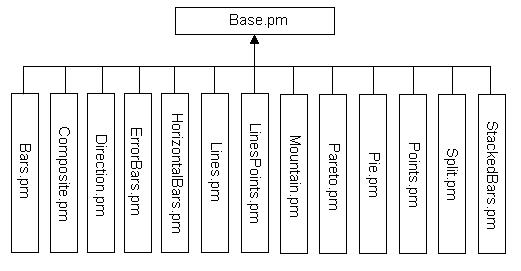
\includegraphics[scale=0.5]{Aufbau.png}
  \end{center}
  \caption{The hierarchy of \class{Chart} classes}
  \label{fig:Aufbau}
\end{figure}

You must create an \emph{instance of one of the concrete subclasses} to
get a \class{Chart} object. Take a look at the individual class
descriptions to see how they work.

All the methods and most of the options \class{Chart} provides are
implemented in the \class{Chart::Base} class. However, drawing of the
graph itself happens in the appropriate subclass.
Figure~\ref{fig:Elemente} shows the elements of a chart from a layout
perspective.

\begin{figure}[ht]
  \begin{center}
    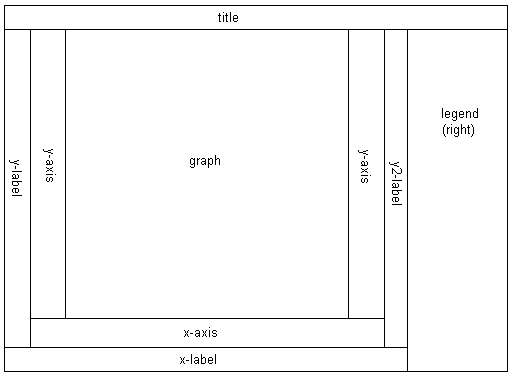
\includegraphics[scale=0.4]{Elemente.png}
  \end{center}
  \caption{Layout Elements of a chart}
  \label{fig:Elemente}
\end{figure}

The graph area in the middle is drawn by the subclass, all the other
elements are drawn by \class{Chart::Base}. But some classes do not need
all of those elements, or they may need additional elements. The
\class{Chart::Base} methods producing these elements have then to be
overwritten in the respective subclass. For example, class
\class{Chart::Pie} needs no axes, so the methods for drawing these in
file Base.pm are overwritten by methods in class \class{Chart::Pie}; in
this case, no axes are drawn. Furthermore, the legend in a pie chart is
slightly different. Therefore, Pie.pm has its own methods for drawing
the legends. All these rules are managed by \class{Chart}, so you do not
have to attend to it.

\class{Chart} uses Lincoln Stein's GD module for all its graphics
primitives calls. So you need an installed version of GD.pm to use
\class{Chart}. This module is available in the CPAN online archive at
\texttt{http://www.cpan.org/}, just like \class{Chart} itself.
\index{GD (module by Lincoln Stein)}

The table lists all attributes that are currently used within the Chart
package. It shows which of the concrete subclasses uses each attribute.

{
\begin{sidewaystable}
\tiny
\begin{tabular}{|l|c|c|c|c|c|c|c|c|c|c|c|c|c|}
\hline
Attribute & Bars& Composite& Direction& ErrorBars& HorizontalBars& Lines& LinesPoints& Mountain& Pareto& Pie& Points& Split& StackedBars \\
\hline
angle\_interval        &   &   & X &   &   &   &   &   &   &   &   &   &   \\
arrow                  &   &   & X &   &   &   &   &   &   &   &   &   &   \\
brush\_size            &   &   & X & X &   & X & X &   &   &   &   &   &   \\
brush\_size1           &   & X &   &   &   &   &   &   &   &   &   &   &   \\
brush\_size2           &   & X &   &   &   &   &   &   &   &   &   &   &   \\
brushStyle             &   &   &   &   &   &   & X &   &   &   & X &   &   \\
brushStyle1            &   & X &   &   &   &   &   &   &   &   &   &   &   \\
brushStyle2            &   & X &   &   &   &   &   &   &   &   &   &   &   \\
colors                 & X & X & X & X & X & X & X & X & X & X & X & X & X \\
composite\_info        &   & X &   &   &   &   &   &   &   &   &   &   &   \\
custom\_x\_ticks       & X & X & X & X & X & X & X & X & X & X & X & X & X \\
f\_x\_tick             & X & X & X & X & X & X & X & X & X & X & X & X & X \\
f\_y\_tick             & X & X & X & X & X & X & X & X & X & X & X & X & X \\
f\_y\_tick1            &   & X &   &   &   &   &   &   &   &   &   &   &   \\
f\_y\_tick2            &   & X &   &   &   &   &   &   &   &   &   &   &   \\
graph\_border          & X & X & X & X & X & X & X & X & X & X & X & X & X \\
grey\_background       & X & X & X & X & X & X & X & X & X & X & X & X & X \\
grid\_lines            & X & X & X & X & X & X & X & X & X & X & X & X & X \\
imagemap               & X & X & X & X & X & X & X & X & X & X & X & X & X \\
include\_zero          & X & X & X & X & X & X & X & X & X & X & X & X & X \\
integer\_ticks\_only   & X & X & X & X & X & X & X & X & X & X & X & X & X \\
interval               &   &   &   &   &   &   &   &   &   &   &   & X &   \\
interval\_ticks        &   &   &   &   &   &   &   &   &   &   &   & X &   \\
label\_font            & X & X & X & X & X & X & X & X & X & X & X & X & X \\
label\_values          &   &   &   &   &   &   &   &   &   & X &   &   &   \\
legend                 & X & X & X & X & X & X & X & X & X & X & X & X & X \\
legend\_example\_height&   & X &   &   &   &   &   &   &   &   &   &   &   \\
legend\_example\_size  & X & X & X & X & X & X & X & X & X & X & X & X & X \\
legend\_font           & X & X & X & X & X & X & X & X & X & X & X & X & X \\
legend\_label\_values  &   &   &   &   &   &   &   &   &   & X &   &   &   \\
legend\_labels         & X & X & X & X & X & X & X & X & X & X & X & X & X \\
legend\_lines          &   &   &   &   &   &   &   &   &   & X &   &   &   \\
line                   &   &   & X &   &   &   &   &   &   &   &   &   &   \\
max\_circles           &   &   & X &   &   &   &   &   &   &   &   &   &   \\
max\_val               & X & X & X & X & X & X & X & X & X & X & X & X & X \\
max\_val1              &   & X &   &   &   &   &   &   &   &   &   &   &   \\
max\_val2              &   & X &   &   &   &   &   &   &   &   &   &   &   \\
max\_x\_ticks          & X & X & X & X & X & X & X & X & X & X & X & X & X \\
max\_y\_ticks          & X & X & X & X & X & X & X & X & X & X & X & X & X \\
min\_circles           &   &   & X &   &   &   &   &   &   &   &   &   &   \\
min\_val               & X & X & X & X & X & X & X & X & X & X & X & X & X \\
min\_val1              &   & X &   &   &   &   &   &   &   &   &   &   &   \\
min\_val2              &   & X &   &   &   &   &   &   &   &   &   &   &   \\
min\_x\_ticks          & X & X & X & X & X & X & X & X & X & X & X & X & X \\
min\_y\_ticks          & X & X & X & X & X & X & X & X & X & X & X & X & X \\
no\_cache              & X & X & X & X & X & X & X & X & X & X & X & X & X \\
pairs                  &   &   & X &   &   &   &   &   &   &   &   &   &   \\
png\_border            & X & X & X & X & X & X & X & X & X & X & X & X & X \\
point                  &   &   & X &   &   &   &   &   &   &   &   &   &   \\
precision              & X & X & X & X & X & X & X & X & X & X & X & X & X \\
pt\_size               &   &   & X & X &   &   & X &   &   &   & X &   &   \\
ring                   &   &   &   &   &   &   &   &   &   & X &   &   &   \\
same\_error            &   &   &   & X &   &   &   &   &   &   &   &   &   \\
same\_y\_axes          &   & X &   &   &   &   &   &   &   &   &   &   &   \\
scale                  &   &   &   &   &   &   &   &   &   &   &   & X &   \\
skip\_int\_ticks       & X & X & X & X & X & X & X & X & X & X & X & X & X \\
skip\_x\_ticks         & X & X & X & X & X & X & X & X & X & X & X & X & X \\
skip\_y\_ticks         &   &   &   &   & X &   &   &   &   &   &   &   &   \\
sort                   &   &   & X & X &   & X & X &   & X &   & X & X &   \\
spaced\_bars           & X &   &   &   & X &   &   &   & X &   &   &   & X \\
start                  &   &   &   &   &   &   &   &   &   &   &   & X &   \\
stepline               &   &   &   &   &   & X & X &   &   &   &   &   &   \\
stepline\_mode         &   &   &   &   &   & X & X &   &   &   &   &   &   \\
sub\_title             & X & X & X & X & X & X & X & X & X & X & X & X & X \\
text\_space            & X & X & X & X & X & X & X & X & X & X & X & X & X \\
tick\_label\_font      & X & X & X & X & X & X & X & X & X & X & X & X & X \\
tick\_len              & X & X & X & X & X & X & X & X & X & X & X & X & X \\
title                  & X & X & X & X & X & X & X & X & X & X & X & X & X \\
title\_font            & X & X & X & X & X & X & X & X & X & X & X & X & X \\
transparent            & X & X & X & X & X & X & X & X & X & X & X & X & X \\
x\_grid\_lines         & X & X & X & X & X & X & X & X & X & X & X & X & X \\
x\_label               & X & X & X & X & X & X & X & X & X & X & X & X & X \\
x\_ticks               & X & X & X & X & X & X & X & X & X & X & X & X & X \\
xlabels                &   &   &   & X &   & X & X &   &   &   & X &   &   \\
xrange                 &   &   &   & X &   & X & X &   &   &   & X &   &   \\
xy\_plot               &   &   &   & X &   & X & X &   &   &   & X &   &   \\
y\_axes                & X &   &   & X & X &   & X & X & X &   & X & X & X \\
y\_grid\_lines         & X & X & X & X & X & X & X & X & X & X & X & X & X \\
y\_label               & X & X & X & X & X & X & X & X & X & X & X & X & X \\
y\_label2              & X & X & X & X & X & X & X & X & X & X & X & X & X \\
y\_ticks               & X & X & X & X & X & X & X & X & X & X & X & X & X \\
y\_ticks1              &   & X &   &   &   &   &   &   &   &   &   &   &   \\
y\_ticks2              &   & X &   &   &   &   &   &   &   &   &   &   &   \\
ylabel2                & X & X & X & X & X & X & X & X & X & X & X & X & X \\
\hline
\end{tabular}
\end{sidewaystable}
}


%\include{example}
%
% Base.tex
%
\renewcommand{\thisname}{Chart::Base}
\section{\thisname}
\name{\thisname}
\file{Base.pm}
\requires{GD, Carp, FileHandle}
\begin{Description}
\thisclass is the abstract superclass of classes \class{Chart::Bars},
\class{Chart::Composite}, \class{Chart::Direction},
\class{Chart::ErrorBars}, \class{Chart::HorizontalBars},
\class{Chart::Lines}, \class{Chart::LinesPoints},
\class{Chart::Mountain}, \class{Chart::Pareto}, \class{Chart::Pie},
\class{Chart::Points}, \class{Chart::Split}, and
\class{Chart::StackedBars}.

Class \thisclass provides all public methods and most of the
attributes of \chart objects.
\end{Description}

\begin{Constructor}
An object instance of class \class{Chart} can be created with the
constructor \methoduse{new()}:\index{Methods!new()}
\begin{SmallExample}
\$obj = Chart::\textit{Type}\deref new();\\
\$obj = Chart::\textit{Type}\deref new(\parameter{width}, \parameter{height});
\end{SmallExample}
\textit{Type} here denotes the type of chart that is to be returned,
\eg, \methoduse{Chart::Bars\deref new()} returns a bar chart.

If \methoduse{new()} is called without arguments, the constructor will
return an object of size 300\ensuremath{\times}400 pixels. If
\methoduse{new()} is called with two arguments, \parameter{width} and
\parameter{height}, it will return a \chart object of the desired
size.
\end{Constructor}


\Methods\label{methods}\noindent%
\methoduse{\$obj\deref add\_dataset(\parameter{@array})}{\index{Methods!add\_dataset()}}\\
\begin{MethDecl}{\$obj\deref add\_dataset(\parameter{\bs @array\_ref})}{add\_dataset()}
Adds a dataset to the object. The argument is an array or a reference to
an array. Generally, the first array added is interpreted as being the
$x$ tick labels. The subsequent arrays contain the data points. \Eg,
after the calls\\
\methoduse{\$obj\deref add\_dataset('Harry', 'Sally');}\\
\methoduse{\$obj\deref add\_dataset(5, 8);}\\
\chart will draw a picture with two bars and label them `Harry' and
`Sally'.

Some modules will operate slightly differently. Have a look at the
description of the specific subclass to get more information. Such
differences will also come up if you want to use the \texttt{xy\_plot}
option in order to create a $x$--$y$ graph.
\end{MethDecl}

\methoddecl{\$obj\deref add\_pt(\parameter{@array})}{add\_pt()}
\begin{MethDecl}{\$obj\deref add\_pt(\parameter{\bs @array\_ref})}{add\_pt()}
This is a different method for adding data to a
\chart object. The argument can be an array or a reference to an
array. If you use this method, \chart wants the complete data of
one data point, \ie, all the data that are associated with the same $x$
value specified first in this call. \Eg,\\
\methoduse{\$obj\deref add\_pt('Harry', 5);}\\
\methoduse{\$obj\deref add\_pt('Sally', 8);}\\
would create the same graph as the example for \methoduse{add\_dataset()} above.
\end{MethDecl}

\methoddecl{\$obj\deref add\_datafile("\parameter{filename}",   \textit{type})}{add\_datafile()}
\methoddecl{\$obj\deref add\_datafile(\parameter{\$filehandle}, \textit{type})}{add\_datafile()}
\begin{MethDecl}{\$obj\deref add\_datafile()}{add\_datafile()}
This method adds the contents of a complete data file to the chart object.
\textit{type} can be \literal{set} or \literal{pt}.
In the former case, \literal{set}, each line in the data file must
represent a complete data set (\emph{data series}). The values of the set
must be separated by whitespace. \Eg, the file contents could look like
this:
\begin{quote}
\texttt{Harry  Sally}\\
\texttt{3      8}\\
\texttt{2      1}
\end{quote}

If the argument is \literal{pt}, the lines of the file must look
analogous to the parameter arrays used by method \methoduse{add\_pt()}:
Each line includes all the values of one data point (\ie, all the $y$
values associated with the same $x$ value), also separated by
whitespace. \Eg:
\begin{quote}
\small
\texttt{Harry 3 2}\\
\texttt{Sally 8 1}
\end{quote}
\end{MethDecl}

\begin{MethDecl}{\$obj\deref get\_data()}{get\_data()}
If you want a copy of the data that have been added
so far, make a call to this method like so:\\
\methoduse{\$dataref = \$obj\deref get\_data();}\\[\itemabstand]
This will return a reference to an array of references to
datasets. For example, you can get the $x$ tick labels by:\\
\methoduse{@x\_labels = @\{\$dataref->[0]\};}
\end{MethDecl}

\begin{MethDecl}{\$obj\deref clear\_data()}{clear\_data()}
This is the method to remove all data that may have been entered until now.
\end{MethDecl}

\methoddecl{\$obj\deref set(\parameter{attribute$_1$} \fatcomma \parameter{value$_1$}, \ldots, \mbox{\parameter{attribute$_n$} \fatcomma \parameter{value$_n$}})}{set()}
\methoddecl{\$obj\deref set(\parameter{\%hash})}{set()}
\methoddecl{\$obj\deref set(\parameter{attribute1}, \parameter{value$_1$}, \ldots, \mbox{\parameter{attribute$_n$}, \parameter{value$_n$}})}{set()}
\begin{MethDecl}{\$obj\deref set(\parameter{@array})}{set()}
Use this method to change the attributes of the chart object.
\methoduse{set()} looks for a hash of keys and values or an array of
keys and values. \Eg,\\
\methoduse{\$obj\deref set('title' \fatcomma 'The title of the image');}\\
would set the title. This would do the same job:\\
\methoduse{\%hash = ('title' \fatcomma 'The title of the image');}\\
\methoduse{\$obj\deref set(\%hash);}
\end{MethDecl}

\methoddecl{\$obj\deref png("\parameter{filename}")}{png()}
\methoddecl{\$obj\deref png(\$\parameter{filehandle})}{png()}
\methoddecl{\$obj\deref png(\parameter{FILEHANDLE})}{png()}
\methoddecl{\$obj\deref png("\parameter{filename}", \parameter{\bs@data})}{png()}
\begin{MethDecl}{\$obj\deref png()}{png()}
This method creates a \textsc{png} file.
The file parameter can be a file name, a reference to a filehandle or a
filehandle itself. If the file does not exist, \chart will
create it for you. If there is already a file, \chart will
overwrite it. In case of an error, the file is not created.\\
You can also add data to a \chart object through its
\methoduse{png()} method. The \parameter{@data} array should contain
references to arrays of data, with the first array reference pointing
to an array of $x$ labels. \parameter{@data} might look like this:\\
\methoduse{@data = (['Harry', 'Sally'], [5, 8], [50, 80]);}\\
This would set up a graph with two datasets and three data points in
these sets.
\end{MethDecl}

\methoddecl{\$obj\deref jpeg("\parameter{filename}")}{jpeg()}
\methoddecl{\$obj\deref jpeg(\parameter{\$filehandle})}{jpeg()}
\methoddecl{\$obj\deref jpeg(\parameter{FILEHANDLE})}{jpeg()}
\methoddecl{\$obj\deref jpeg("\parameter{filename}", \bs@data)}{jpeg()}
\begin{MethDecl}{\$obj\deref jpeg()}{jpeg()}
This is the method to create \textsc{jpeg} files. It works analogously
to the \methoduse{png()} method.
\end{MethDecl}

\methoddecl{\$obj\deref cgi\_png()}{cgi\_png()}
\begin{MethDecl}{\$obj\deref cgi\_jpeg()}{cgi\_jpeg()}
With the \textsc{cgi} methods you can create dynamic images for your web
site. The \textsc{cgi} methods will print the chart along with the
appropriate \textsc{http} header to \textsc{stdout}, allowing you to
call chart-generating scripts directly from your \textsc{html} pages
(\eg, with a \literal{$\langle$img src="image.pl" /$\rangle$}
\textsc{html} tag).
\end{MethDecl}

\begin{MethDecl}{\$obj\deref imagemap\_dump()}{imagemap\_dump()}
\chart can also return pixel position information so that you can
create image maps from the files generated by \chart. Simply set the
\literal{imagemap} option to \literal{true} before you generate the
file, then at the end call the \methoduse{imagemap\_dump()} method to
retrieve the information. A structure will be returned almost identical
to the \parameter{@data} array described above to pass the data into \chart.

\methoduse{\$imagemap\_data = \$obj\deref imagemap\_dump();}

Instead of single data values, references to arrays of pixel information
are passed. For the classes \class{Chart::Bars},
\class{Chart::HorizontalBars}, \class{Chart::Pareto} and
\class{Chart::StackedBars}, the arrays will contain two $x$--$y$ pairs
(specifying the upper left and the lower right corner of the bar).
Compare to: \\
\methoduse{(\$x1,\$y1,\$x2,\$y2) = @\{\$imagemap\_data\deref [\$dataset][\$datapoint]\};}

For the classes \class{Chart::Lines}, \class{Chart::Points},
\class{Chart::LinesPoints} and \class{Chart::Split}, the arrays will
contain a single $x$--$y$ pair (specifying the center of the point).
Compare to:\\
\methoduse{(\$x, \$y) = @\{\$imagemap\_data\deref [\$dataset][\$datapoint]\};}

A few caveats apply here. First of all, \chart uses the GD module by
Lincoln Stein to draw lines, circles, strings, and so on. GD treats the
upper-left corner of the \textsc{png}/\textsc{jpeg} image as the
reference point, therefore, positive $y$ values are measured from the
top of the image, not from the bottom. Second, these values will mostly
contain long decimal values. GD, of course, has to truncate these to
integer pixel coordinates. In a worst-case scenario, this will result in
an error of one pixel on your imagemap. If this is really an issue, your
only option is to experiment with it, or to contact Lincoln Stein and
ask him. Third, please remember that the $0^{th}$ dataset will be empty,
since that is the place for the data point labels on the $x$ axis.
\end{MethDecl}


\Attributes\label{options}%
These are the options which take effect on most \chart types.
There are three different kinds of attributes:
\begin{itemize}
\item attributes expecting a number for value (\eg, the number of pixels),
\item attributes expecting a textual value (\eg, the title of the chart),
\item attributes expecting a Boolean value.
\end{itemize}

Before Version 2.5 of the module, the Boolean value \literal{true} was
represented by the string \texttt{'true'}, and the Boolean value
\literal{false} was represented by the string \texttt{'false'}. For all
other values, the Boolean value was not well-defined.
From version 2.5 onwards, the Boolean value \literal{true} may be
represented by any of \texttt{1}, \texttt{'t'} and \texttt{'true'},
where case does not matter.
From version 2.5 onwards, the Boolean value \literal{false} may be
represented by any of \texttt{0}, \texttt{'f'}, \texttt{'false'}, and
\texttt{undef}, where case does not matter. For all other values, the
Boolean value is again not well-defined. Note that this behaviour is
closer to the standard Perl way but is not identical, due to the need
for backward compatibility in this module.

\begin{AttrDecl}{transparent}
Makes the background of the image transparent if set to \literal{true}.
Useful for making web page images. However, it does not seem to work
for all browsers. Defaults to \literal{false}.
\end{AttrDecl}

\begin{AttrDecl}{png\_border}
Sets the number of pixels used as a border between the graph and the
edges of the image. Defaults to 10.
\end{AttrDecl}

\begin{AttrDecl}{graph\_border}
Sets the number of pixels used as a border between the title/labels and
the actual graph within the image. Defaults to 10.
\end{AttrDecl}

\begin{AttrDecl}{text\_space}
Sets the amount of space left on the sides of text, to make it more
readable. Defaults to 3.
\end{AttrDecl}

\begin{AttrDecl}{title}
Tells \chart what to use for the title of the graph. If empty, no title
is drawn. \literal{\bs\bs} is treated as a newline. If you want to use
normal quotation marks instead of single quotation marks, remember to
quote (\literal{\bs\bs\bs\bs}) to get a linebreak. Default is empty.
\end{AttrDecl}

\begin{AttrDecl}{sub\_title}
Writes a subtitle under the title in smaller letters.
\end{AttrDecl}

\begin{AttrDecl}{x\_label}
Tells \chart what text to use as a label for the $x$ axis. If empty, no
label is drawn. Default is undef.
\end{AttrDecl}

\attrdecl{y\_label}
\begin{AttrDecl}{y\_label2}
Tells \chart what kind of label should be used for the description of
the $y$ axis on the left or the right side accordingly. If empty, no
label is drawn.  Default is undef.
\end{AttrDecl}

\begin{AttrDecl}{legend}
Specifies the placement of the legend. Valid values are
\literal{left}, \literal{right}, \literal{top},
\literal{bottom}, and \literal{none}. Choosing \literal{none}
tells \chart not to draw a legend. Default is \literal{right}.
\end{AttrDecl}

\begin{AttrDecl}{legend\_labels}
Sets the values for the labels for the different datasets. Should be
assigned a reference to an array of labels. \Eg,\\
\methoduse{@labels = ('foo', 'bar')};\\
\methoduse{\$obj->set ('legend\_labels' \fatcomma \bs @labels);}\\
Default is empty, in which case \literal{Dataset 1},
\literal{Dataset 2}, etc. are used as labels.
\end{AttrDecl}

\begin{AttrDecl}{tick\_len}
Sets the length of the $x$ and $y$ ticks in pixels. Default is 4.
\end{AttrDecl}

\begin{AttrDecl}{x\_ticks}
Specifies how to draw the $x$ tick labels. Valid values are
\literal{normal}, \literal{staggered} (labels are drawn alternatingly
close to the axis and further away from it), and \literal{vertical}
(label texts are rotated 90 degrees counter-clockwise). Default is
\literal{normal}.
\end{AttrDecl}

\begin{AttrDecl}{y\_ticks}
The number of ticks to plot on the $y$ scale, including the end points.
\Eg, for a $y$ axis ranging from 0 to 50, with ticks every 10 units,
\attruse{y\_ticks} should have a value of 6.
\end{AttrDecl}

\begin{AttrDecl}{min\_y\_ticks}
Sets the minimum number of $y$ ticks to draw when generating the $y$
axis. Default is 6, minimum is 2.
\end{AttrDecl}

\begin{AttrDecl}{max\_y\_ticks}
Sets the maximum number of $y$ ticks to draw when generating the $y$
axis. Default is 100. This limit is used to avoid plotting an
unreasonably large number of ticks if non-round values are used for
\attruse{min\_val} and \attruse{max\_val}. The value for
\attruse{max\_y\_ticks} should be at least 5 times as large as
\attruse{min\_y\_ticks}.
\end{AttrDecl}

\attrdecl{min\_x\_ticks}
\begin{AttrDecl}{max\_x\_ticks}
These work similar to \attruse{max\_y\_ticks} and
\attruse{min\_y\_ticks}, respectively. Of course, this applies only to
$x$--$y$ plots.
\end{AttrDecl}

\begin{AttrDecl}{integer\_ticks\_only}
Specifies how to draw the $x$ and $y$ ticks: as floating point
(\literal{false}, \literal{0}) or as integer numbers
(\literal{true}, \literal{1}). If you want integer ticks, it may
be better to set the attribute \attruse{precision} to zero. Default:
\literal{false}
\end{AttrDecl}

\begin{AttrDecl}{skip\_int\_ticks}
If \attruse{integer\_ticks\_only} was set to \literal{true} the
labels and ticks for the $y$ axis will be drawn every $n^{th}$ tick.
(Note that in \class{Chart::HorizontalBars} the $y$ axis runs
horizontally.) Defaults to 1, \ie, no skipping.
\end{AttrDecl}

\begin{AttrDecl}{precision}
Sets the number of digits after the decimal point. Affects in most cases
the $y$ axis only. In $x$--$y$ plots also affects the $x$ axis, and in
pie charts the labels. Defaults to 3.
\end{AttrDecl}

\begin{AttrDecl}{max\_val}
Sets the maximum $y$ value on the graph, overriding normal autoscaling.
Does not work for \class{Chart::Split} charts. Default is undef.
\end{AttrDecl}

\begin{AttrDecl}{min\_val}
Sets the minimum $y$ value on the graph, overriding normal autoscaling.
Does not work for Split charts. Default is undef. Caution should be
used when setting \attruse{max\_val} and \attruse{min\_val} to
floating point or non-round numbers: The range must start and end on a
tick, ticks must have round-number intervals and must include round
numbers.\\
Example: Suppose your dataset has a range of 35\ldots 114
units. If you specify these values as \attruse{min\_val} and
\attruse{max\_val}, respectively, the $y$ axis will be plotted with 80
ticks, so one at every unit. Without specification of
\attruse{min\_val} and \attruse{max\_val}, the system would
autoscale the range to 30\ldots 120 with 10 ticks every 10 units. If
\attruse{min\_val} and \attruse{max\_val} are specified to excessive
precision, they may be overridden by the system, plotting a maximum
\attruse{max\_y\_ticks} ticks.
\end{AttrDecl}

\begin{AttrDecl}{include\_zero}
If \literal{true}, forces the $y$ axis to include zero even if it is
not in the dataset range. Default is \literal{false}. -- Note:
It is better to use this option than to set \attruse{min\_val}
if this is all you want to achieve.
\end{AttrDecl}

\begin{AttrDecl}{skip\_x\_ticks}
Sets the number of $x$ ticks and $x$ tick labels to skip. (\Ie, if
\attruse{skip\_x\_ticks} were set to 4, \chart would draw every
$4^{th}$ $x$ tick and $x$ tick label). Default is undef.
\end{AttrDecl}

\begin{AttrDecl}{custom\_x\_ticks}
This option allows you to specify exactly which $x$ ticks and $x$ tick
labels should be drawn. It should be assigned a reference to an array of
desired ticks. Just remember that we are counting from the $0^{th}$
element of the array. (\Eg, if \attruse{custom\_x\_ticks} is assigned
[0,3,4], then the $0^{th}$, $3^{rd}$, and $4^{th}$ $x$ ticks will be
displayed) This does not apply to \class{Chart::Split},
\class{Chart::HorizontalBars} and \class{Chart::Pie}.
\end{AttrDecl}

\begin{AttrDecl}{f\_x\_tick}
Needs a reference to a function which accepts the $x$ tick labels
generated by \parameter{\$data\deref [0]} as its argument. This function
should return a reformatted version of the label as a string. \Eg\\
\methoduse{\$obj\deref set ('f\_x\_tick' \fatcomma \bs\&formatter;})\\
An example for the formatter function: Assume that $x$ labels are
seconds since some event. The referenced function could be designed to
transform this number of seconds to hours, minutes and seconds.
\end{AttrDecl}

\begin{AttrDecl}{f\_y\_tick}
Similar to \attruse{f\_x\_tick}, but for $y$ labels.
\end{AttrDecl}

\begin{AttrDecl}{colors}
\label{colors}
This option lets you control the colors the chart will use. It takes a
reference to a hash. The hash should contain keys mapped to references
to arrays of \textsc{rgb} values. E.g.,\\
\methoduse{\$obj->set('colors' \fatcomma \{'background' \fatcomma [255,255,255]\});}\\
sets the background color to white (which is the default).\\
Another possibility is to use named colors like 'red', 'blue'. The possible
list of named colors can be found in chapter \ref{app:colors}, page \pageref{app:colors}.\\ 
Valid keys for this hash are
\begin{itemize}
\item \literal{background} (background color for the chart)
\item \literal{title} (color of the title)
\item \literal{text} (all the text in the chart)
\item \literal{x\_label} (color of the $x$ axis label)
\item \literal{y\_label} (color of the primary $y$ axis label)
\item \literal{y\_label2} (color of the secondary $y$ axis label)
\item \literal{grid\_lines} (color of the grid lines)
\item \literal{x\_grid\_lines} (color of the $x$ grid lines -- on $x$ axis ticks)
\item \literal{y\_grid\_lines} (color of the $y$ grid lines -- on primary $y$ axis ticks)
\item \literal{y2\_grid\_lines} (color of the y2 grid lines -- on secondary $y$ axis ticks)
\item \literal{dataset0} \ldots \literal{dataset63} (the different datasets)
\item \literal{misc} (everything else, \eg, ticks, box around the legend)
\end{itemize}

NB. For composite charts, there is a limit of eight datasets per
component. The colors for \literal{dataset8} through \literal{dataset15}
will be the same as those for \literal{dataset0} through
\literal{dataset7} for the second component chart.
\end{AttrDecl}

\begin{AttrDecl}{title\_font}
This option changes the font of the title line. The value must be a GD
font, \eg, \methoduse{GD::Font\deref Large}.
\end{AttrDecl}

\begin{AttrDecl}{label\_font}
This option changes the font of the labels. The value must be a GD font.
\end{AttrDecl}

\begin{AttrDecl}{legend\_font}
This option changes the font for the legend text. The value must be a
GD font.
\end{AttrDecl}

\begin{AttrDecl}{tick\_label\_font}
This option changes the font of the ticks. The value must be a GD font.
\end{AttrDecl}

\begin{AttrDecl}{grey\_background}
Puts a nice soft grey background on the actual data plot when set to
\literal{true}. This is a flag. If you set this flag to 'false' then you may
redefine the background color to a color you like. For further information see chapter \ref{colors}
on page \pageref{colors}. Default is \literal{true}.
\end{AttrDecl}

\begin{AttrDecl}{x\_grid\_lines}
Draws grid lines matching up to $x$ ticks if set to \literal{true}.
Default is \literal{false}.
\end{AttrDecl}

\begin{AttrDecl}{y\_grid\_lines}
Draws grid lines matching up to $y$ ticks if set to \literal{true}.
Default is \literal{false}.
\end{AttrDecl}

\begin{AttrDecl}{grid\_lines}
Draws grid lines matching up to $x$ and $y$ ticks if set to
\literal{true}. Default is \literal{false}.
\end{AttrDecl}

\begin{AttrDecl}{imagemap}
Lets \chart know that you are going to ask for information about the
placement of the data for use in creating an image map from the chart.
This information can be retrieved using the
\mbox{\methoduse{imagemap\_dump()}}
method. NB. The \methoduse{imagemap\_dump()} method cannot be called
until after the chart has been generated (\eg, using the \methoduse{png()}
or \methoduse{cgi\_png()} methods).
\end{AttrDecl}

\begin{AttrDecl}{ylabel2}
The label for the secondary (right-hand side) $y$ axis. (In a composite
chart, this is the axis for the second component). Default is undef.
\end{AttrDecl}

\begin{AttrDecl}{no\_cache}
Adds \literal{Pragma: no-cache} to the \textsc{http} header.
Be careful with this one, since some older browsers (like Netscape~4.5)
are unhappy about \textsc{post} using this method.
\end{AttrDecl}

\begin{AttrDecl}{legend\_example\_size}
Sets the length of the example line in the legend. Defaults to 20.
\end{AttrDecl}


%
% bars.tex
%
\renewcommand{\thisname}{Chart::Bars}
\section{\thisname}
\name{\thisname}
\file{Bars.pm}
\requires{Chart::Base, GD, Carp, FileHandle}
\begin{Description}
The class \thisclass creates a chart made up of vertical bars.
\thisclass is a subclass of \class{Chart::Base}.
\end{Description}

\example
\begin{figure}[ht]
  \begin{center}
    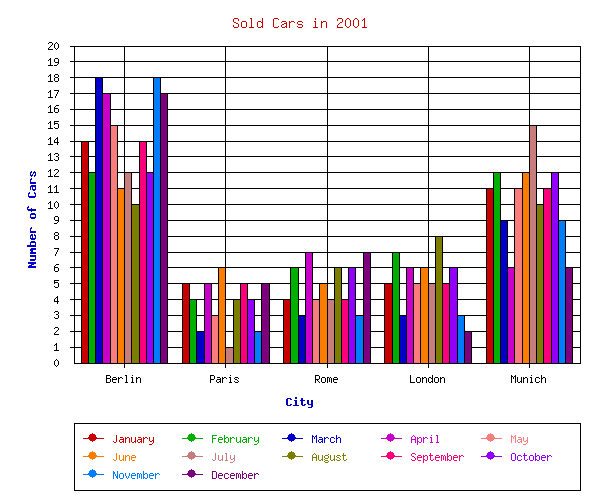
\includegraphics[scale=0.4]{d_bars.png}
  \end{center}
  \caption{Bar chart}
  \label{fig:bars}
\end{figure}

{\small
\begin{verbatim}
use Chart::Bars;

$g = Chart::Bars->new(600,500);

$g->add_dataset('Berlin', 'Paris', 'Rome', 'London', 'Munich');
$g->add_dataset(14, 5, 4, 5, 11);
$g->add_dataset(12, 4, 6, 7, 12);
$g->add_dataset(18, 2, 3, 3, 9);
$g->add_dataset(17, 5, 7, 6, 6);
$g->add_dataset(15, 3, 4, 5, 11);
$g->add_dataset(11, 6, 5, 6, 12);
$g->add_dataset(12, 1, 4, 5, 15);
$g->add_dataset(10, 4, 6, 8, 10);
$g->add_dataset(14, 5, 4, 5, 11);
$g->add_dataset(12, 4, 6, 6, 12);
$g->add_dataset(18, 2, 3, 3, 9);
$g->add_dataset(17, 5, 7, 2, 6);

%hash = ('title' => 'Sold Cars in 2001',
         'text_space'         => 5,
         'grey_background'    => 'false',
         'integer_ticks_only' => 'true',
         'x_label'            => 'City',
         'y_label'            => 'Number of Cars',
         'legend'             => 'bottom',
         'legend_labels'      => ['January',  'February', 
                                  'March',    'April',
                                  'May',      'June', 
                                  'July',     'August',
                                  'September','October', 
                                  'November', 'December'
                                 ],
         'min_val'            => 0,
         'max_val'            => 20,
         'grid_lines'         =>'true',
         'colors'             => {'title'   => 'red',
                                  'x_label' => 'blue',
                                  'y_label' => 'blue'
                                 }
        );

$g->set(%hash);

$g->png("bars.png");
\end{verbatim}
}

\constructorblurb{\thisname}

\begin{AttrDecl}{spaced\_bars}
Leaves some space between each group of bars when set to \literal{true}.
This usually make it easier to read a bar chart. Default is
\literal{true}.
\end{AttrDecl}

\begin{AttrDecl}{y\_axes}
Tells \thisclass where to place the $y$ axis. Valid values are
\literal{left}, \literal{right} and \literal{both}. Defaults to
\literal{left}.
\end{AttrDecl}

% composite.tex
%
\renewcommand{\thisname}{Chart::Composite}
\section{\thisname}
\name{\thisname}
\file{Composite.pm}
\requires{Chart::Base, GD, Carp, FileHandle}
\begin{Description}
The class \thisclass creates a two component chart with two types of
charts which are layered one above each other. Just set the option
\attruse{composite\_info}. For example, you can create a two component
chart with bars and lines. A composite chart does not make sense with
all combinations of chart types, but it works pretty good with Lines,
Points, LinesPoints and Bars. Note that two similar chart types may come
into visual conflict. \thisclass can do only composite charts made up of
two components. \thisclass is a subclass of \class{Chart::Base}.
\end{Description}

\example
\begin{figure}[ht]
  \begin{center}
    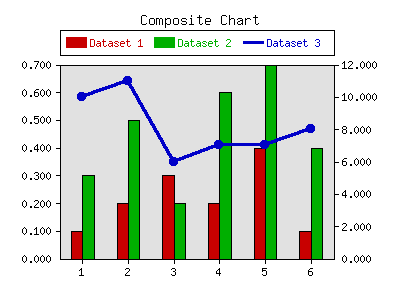
\includegraphics[scale=0.6]{composite.png}
  \end{center}
  \caption{Composite chart}
  \label{fig:composite}
\end{figure}
\begin{verbatim}
use Chart::Composite;

$g = Chart::Composite->new();

$g->add_dataset(1, 2, 3, 4, 5, 6);
$g->add_dataset(0.1, 0.2, 0.3, 0.2, 0.4, 0.1);
$g->add_dataset(0.3, 0.5, 0.2, 0.6, 0.7, 0.4);
$g->add_dataset(10,  11,  6,   7,   7,   8);

$g->set('composite_info' => [ ['Bars',        [1, 2]],
                              ['LinesPoints', [3]  ]
                            ],
        'title'                     => 'Composite Chart',
        'legend'                    => 'top',
        'legend_example_height'     => 'true',
        'legend_example_height0..1' => 10,
        'legend_example_height2'    =>  3,
       );
$g->set('include_zero'  => 'true');

$g->png("composite.png");
\end{verbatim}

\constructorblurb{\thisname}

\attrdecl{brush\_size1}
\begin{AttrDecl}{brush\_size2}
If using component charts having \attruse{brush\_size} as one of their
attributes, you can define the sizes of the brushes individually.
Default is 6 (pixel).
\end{AttrDecl}

\begin{AttrDecl}{composite\_info}
This option is only used for composite charts. It contains the
information which types to use for the two component charts, and which
datasets belong to which component chart. It should be a reference to an
array of array references, containing information like the following:\\
\$obj\deref set ('composite\_info' \fatcomma [ ['Bars', [1,2]], ['Lines', [3,4] ] ]);

This example would set the two component charts to be a bar chart and a
line chart. It would use the first two data sets for the bar chart and
the second two data sets for the line chart. The default is undef. Note
that the numbering starts at 1, not at 0 like most of the other numbered
things in \class{Chart}, because index 0 refers to the $x$ values which
are shared by the two component charts. The ordering of the components
may be important, since the first component is drawn first and then
(partially) overdrawn with the second component. \Eg, when composing a
line graph and a bar graph, it is safer to have the bars in the first
component since otherwise the line(s) might be hidden behind them.
\end{AttrDecl}

\attrdecl{f\_y\_tick1}
\begin{AttrDecl}{f\_y\_tick2}
Needs a reference to a function which uses the $y$ tick labels for the
primary and for the secondary $y$ axis, respectively. These functions
should return a reformatted version of the label as a string. \Eg
\begin{SmallExample}
\$obj\deref set ('f\_y\_tick1' \fatcomma \bs\&formatter1);\\
\$obj\deref set ('f\_y\_tick2' \fatcomma \bs\&formatter2);
\end{SmallExample}
\end{AttrDecl}

\attrdecl{max\_val1}
\begin{AttrDecl}{max\_val2}
Only for composite charts. These options specify the maximum $y$ value
for the first and the second component, respectively. Both default to
undef.
\end{AttrDecl}

\attrdecl{min\_val1}
\begin{AttrDecl}{min\_val2}
Only for composite charts. These options specify the minimum $y$ value
for the first and the second component, respectively. Both default to
undef.
\end{AttrDecl}

\begin{AttrDecl}{legend\_example\_height}
Only for composite charts. This option changes the thickness of the
lines in the legend. If `legend\_example\_height' is set to `true' the
thickness of each legend line can be changed individually. Default is
false. \Eg
\begin{SmallExample}
\$obj\deref set ('legend\_example\_height'     \fatcomma 'true');\\
\$obj\deref set ('legend\_example\_height0'    \fatcomma '3');\\
\$obj\deref set ('legend\_example\_height1..4' \fatcomma '10');
\end{SmallExample}

This example would set the thickness of the first line in the legend to
3, and the thicknesses of the following 4 lines to 10 (using the same
indexing scheme as in `composite\_info'). The default value for each
individual entry is 1, \ie a `normal' line is drawn. It is not possible
to change a 'legend\_example\_height\#'(where \# denotes a dataset
number) which was once defined. (The first setting will remain
unchanged.)
\end{AttrDecl}

\begin{AttrDecl}{same\_y\_axes}
Forces both component charts in a composite chart to use the same
maximum and minimum $y$ values if set to `true'. This helps to keep
some composite charts from being too confusing. Default is undef.
\end{AttrDecl}

\attrdecl{y\_ticks1}
\begin{AttrDecl}{y\_ticks2}
The number of $y$ ticks to use on the primary and on the secondary $y$
axis on a composite chart, respectively. Please note that if you just
set the `y\_ticks' option, both axes will use that number of $y$ ticks.
Both default to undef.
\end{AttrDecl}

%
% direction.tex
%
\renewcommand{\thisname}{Chart::Direction}
\section{\thisname}
\name{\thisname}
\file{Direction.pm}
\requires{Chart::Base, GD, Carp, FileHandle}
\begin{Description}
The class \thisclass creates a diagram based on polar
coordinates. This type of diagram is occasionally referred to as a
\emph{radial} or as a \emph{radar} chart. \thisclass plots data
specified by angle (\eg, wind direction) and absolute value (\eg, wind
strength). The first dataset to add is always the set of angles in
degrees. The second set contains the absolute values. How additional
datasets should be entered depends on the option \attruse{pairs} (cf.
below). By default, \thisclass will draw a point chart. You can also
get a lines chart by setting the option \attruse{point} to
\literal{false} and the option \attruse{line} to \literal{true}. If you
want a lines and point chart, then set both \attruse{point} and
\attruse{line} to \literal{true}. In addition, \thisclass plots arrows
from the center to the point or to the end of the line if the option
\attruse{arrow} is set to \literal{true}. \thisclass is a subclass of
\class{Chart::Base}.
\end{Description}

\example
\begin{figure}[ht]
  \begin{center}
    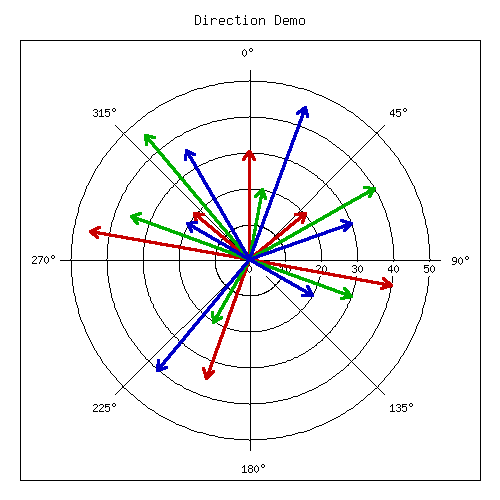
\includegraphics[width = 8cm, height =8cm]{direction.png}
  \end{center}
  \caption{Direction chart}
  \label{fig:direction}
\end{figure}
\begin{verbatim}
use Chart::Direction;
$g = Chart::Direction->new(500,500);

$g->add_dataset( 0, 100, 50, 200, 280, 310);
$g->add_dataset(30,  40, 20,  35,  45,  20);

$g->add_dataset(10, 110, 60, 210, 290, 320);
$g->add_dataset(20,  30, 40,  20,  35,  45);

$g->add_dataset(20, 120, 70, 220, 300, 330);
$g->add_dataset(45,  20, 30,  40,  20,  35,);

%hash = ( 'title'           => 'Direction Demo',
          'angle_interval'  => 45,
          'precision'       => 0,
          'arrow'           => 'true',
          'point'           => 'false',
          'include_zero'    => 'true',
          'pairs'           => 'true',
          'legend'          => 'none',
          'grey_background' => 'false'
        );

$g->set(%hash);

$g->png("direction.png");
\end{verbatim}

\constructorblurb{\thisname}

\begin{AttrDecl}{angle\_interval}
This option tells \thisclass how many angle lines should be drawn. It is
the difference between two angle lines. The default value is 30, which
means that one line will be drawn every 30 degrees. Not all values are
permissible; the valid ones are: 0, 5, 10, 15, 20, 30, 45, and 90. If
you choose 0, \thisclass will draw no lines.
\end{AttrDecl}

\begin{AttrDecl}{arrow}
Draws an arrow from the center of the chart to the point if set to
\literal{true}. By default \literal{false}.
\end{AttrDecl}

\begin{AttrDecl}{brush\_size}
Sets the width of the lines in pixels. Default is 6.
\end{AttrDecl}

\begin{AttrDecl}{line}
Connects the points with lines if set to \literal{true}. Defaults to
\literal{false}.
\end{AttrDecl}

\begin{AttrDecl}{max\_circles}
Sets the maximum number of circles to draw when generating the set of
circles. Default is 100. This limit is used to avoid plotting an
unreasonably large number of circles if non-round values are used for
\attruse{min\_val} and \attruse{max\_val}. The value for
\attruse{max\_circles} should be at least 5 times that of
\attruse{min\_circles}.
\end{AttrDecl}

\begin{AttrDecl}{min\_circles}
Sets the minimum number of circles to draw when generating a scale.
Default is 4, minimum is 2.
\end{AttrDecl}

\begin{AttrDecl}{pairs}
This option tells \thisclass how to handle additional datasets. If
\attruse{pairs} is set to \literal{true}, \thisclass uses the first
dataset as a set of degrees and the second dataset as a set of values.
Then, the third set is a set of degrees and the fourth a set of values,
and so forth. If \attruse{pairs} is set to \literal{false}, \thisclass
uses the first dataset as a set of angles and all following datasets as
sets of values. Defaults to \literal{false}.
\end{AttrDecl}

\begin{AttrDecl}{point}
Indicates to draw points for representing the data values. Possible
values: \literal{true} and \literal{false}, by default \literal{true}.
\end{AttrDecl}

\begin{AttrDecl}{pt\_size}
Sets the radius of the points in pixels. Default is 18.
\end{AttrDecl}

\begin{AttrDecl}{sort}
Sorts the data in ascending order if set to \literal{true}. Should be
set if the input data is not sorted and \attruse{line} is set to
\literal{true}. Defaults to \literal{false}.
\end{AttrDecl}

%
% error.tex
%
\renewcommand{\thisname}{Chart::ErrorBars}
\section{\thisname}
\name{\thisname}
\file{ErrorBars.pm}
\requires{Chart::Base, GD, Carp, FileHandle}

\begin{Description}
The class \thisclass creates a point chart with error bars. This
class expects the error values within the data array. By use of the
\methoduse{add\_dataset()} method the error values are the next two sets
after the $y$ values. The first set after the $y$ values has to be the
set of values for the upper error bounds. The next set is the array of
the lower error bounds. Note that the error values are not specified
absolutely but rather as offsets from the $y$ value: the upper error
values will be added to the $y$ values, the lower error values will be
subtracted.

If you want to use the same value for the upper and lower error, you
can set the \attruse{same\_error} option to \literal{true}. In this
case only the set after the $y$ values is interpreted as a set of
errors.

Of course, it is also possible to use the \methoduse{add\_pt()}
method in the appropriate way to achieve the same results.
\thisclass is a subclass of \class{Chart::Base}.
\end{Description}

\example
\begin{figure}[ht]
  \begin{center}
    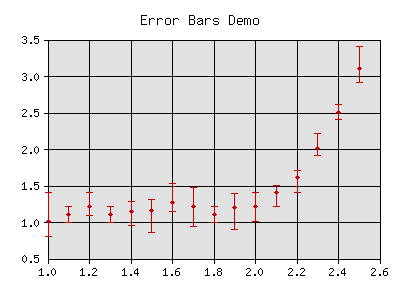
\includegraphics[scale=0.7]{error.png}
  \end{center}
  \caption{Error bars chart}
  \label{fig:error}
\end{figure}

\begin{verbatim}
use Chart::ErrorBars;
$g = Chart::ErrorBars->new();

# the x values
$g->add_dataset(qw(1    1.1  1.2  1.3  1.4  1.5  1.6  1.7
                   1.8  1.9  2    2.1  2.2  2.3  2.4  2.5));
# the y values
$g->add_dataset(qw(1    1.1  1.2  1.1  1.14 1.15 1.26 1.2
                   1.1  1.19 1.2  1.4  1.6  2.0  2.5  3.1));
# the upper errors
$g->add_dataset(qw(0.4  0.1  0.2  0.1  0.14 0.15 0.26 0.27
                   0.1  0.19 0.2  0.1  0.1  0.2  0.1  0.3));
# the lower errors
$g->add_dataset(qw(0.2  0.11 0.12 0.11 0.2  0.3  0.12 0.27
                   0.11 0.3  0.2  0.2  0.2  0.1  0.1  0.2));

$g->set( 'xy_plot'    => 'true',
         'precision'  => 1,
         'pt_size'    => 10,
         'brush_size' => 2,
         'legend'     => 'none',
         'title'      => 'Error Bars Demo',
         'grid_lines' => 'true'
       );

$g->png("errorbars.png");
\end{verbatim}

\constructorblurb{\thisname}

\begin{AttrDecl}{brush\_size}
Sets the width of the lines in pixels. Default is 6.
\end{AttrDecl}

\begin{AttrDecl}{pt\_size}
Sets the radius of the points in pixels. Default is 18.
\end{AttrDecl}

\begin{AttrDecl}{same\_error}
Tells \thisclass that you want to use the same values for
upper and lower error bounds if set to \literal{true}. Then you have to
add just one set of error values. Defaults to \literal{false}.
\end{AttrDecl}

\begin{AttrDecl}{sort}
Sorts the data in ascending order if set to \literal{true}. Should be
set if the input data is not sorted. Defaults to \literal{false}.
\end{AttrDecl}

\attrdecl{xlabels}
\begin{AttrDecl}{xrange}
This pair of options allows arbitrary positioning of $x$ axis labels.
The two options must either both be specified or both be omitted.
\attruse{xlabels} is a reference to 2-element array. The first of the
elements is a nested (reference to an) array of strings that are the
labels. The second element is a nested (reference to an) array of
numbers that are the $x$ values at which the labels should be placed.
\attruse{xrange} is a 2-element array specifying the minimum and maximum
$x$ values on the axis. \Eg,
\begin{verbatim}
@labels = (['Jan', 'Feb', 'Mar'],
           [10,    40,    70   ]);
$chart->set(xlabels => \bs @labels,
            xrange  => [0, 100]
           );
\end{verbatim}
\end{AttrDecl}

\begin{AttrDecl}{xy\_plot}
Forces \thisclass to plot a $x$--$y$ graph if set to \literal{true},
\ie, to treat the $x$ axis as numeric. Very useful for plots of
mathematical functions. Defaults to \literal{false}.
\end{AttrDecl}

\begin{AttrDecl}{y\_axes}
Tells \thisclass where to place the $y$ axis. Valid values are
\literal{left}, \literal{right} and \literal{both}. Defaults to
\literal{left}.
\end{AttrDecl}

%
% hbars.tex
%
\renewcommand{\thisname}{Chart::HorizontalBars}
\section{\thisname}
\name{\thisname}
\file{HorizontalBars.pm}
\requires{Chart::Base, GD, Carp, FileHandle}
\begin{Description}
The class \thisclass creates a chart of horizontally oriented bars.
\thisclass is a subclass of \class{Chart::Base}.
\end{Description}

\example
\begin{figure}[ht]
  \begin{center}
    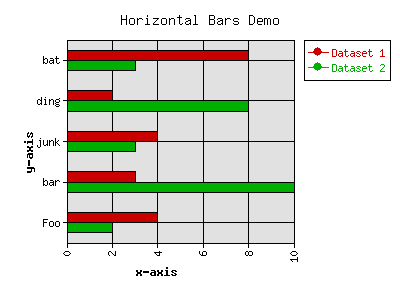
\includegraphics[scale=0.7]{d_hbars4.png}
  \end{center}
  \caption{Chart with horizontal bars}
  \label{fig:hbars}
\end{figure}
\begin{verbatim}
use Chart::HorizontalBars;

$g = Chart::HorizontalBars->new();
$g->add_dataset('Foo', 'bar', 'junk', 'ding', 'bat');
$g->add_dataset(4, 3, 4, 2, 8);
$g->add_dataset(2, 10, 3, 8, 3);

%hash = ( 'title'        => 'Horizontal Bars Demo',
          'grid_lines'   => 'true',
          'x_label'      => 'x axis',
          'y_label'      => 'y axis',
          'include_zero' => 'true',
          'x_ticks'      => 'vertical',
         );
$g->set(%hash);

$g->png("hbars.png");
\end{verbatim}

\constructorblurb{\thisname}

\begin{AttrDecl}{skip\_y\_ticks}
Does the same fo the $y$ axis in a horizontal chart as
\attruse{skip\_x\_ticks} does for other charts. Defaults to 1.
\end{AttrDecl}

\begin{AttrDecl}{spaced\_bars}
Leaves some space between each group of bars when set to \literal{true}. This
usually make it easier to read a bar chart. Default is \literal{true}.
\end{AttrDecl}

\begin{AttrDecl}{y\_axes}
Tells \thisclass where to place the $y$ axis.
\literal{left}, \literal{right} and \literal{both}. Defaults to
\literal{left}.
\end{AttrDecl}

%
% lines.tex
%
\renewcommand{\thisname}{Chart::Lines}
\section{\thisname}
\name{\thisname}
\requires{Chart::Base, GD, Carp, FileHandle}
\begin{Description}
The class \thisclass creates a lines chart. (If you want the data
points marked with symbols, check \class{Chart::LinesPoints} on
page \pageref{Chart::LinesPoints}.) \thisclass is a subclass of
\class{Chart::Base}.
\end{Description}

\example
\begin{figure}[ht]
  \begin{center}
    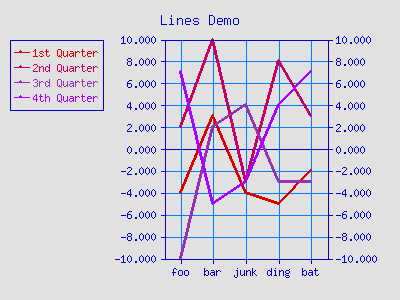
\includegraphics[scale=0.5]{d_lines2.png}
  \end{center}
  \caption{Lines chart}
  \label{fig:lines}
\end{figure}
\begin{verbatim}
use Chart::Lines;

$g = Chart::Lines->new();
$g->add_dataset('foo', 'bar', 'junk', 'ding', 'bat');
$g->add_dataset( -4,  3, -4, -5, -2);
$g->add_dataset(  2, 10, -3,  8,  3);
$g->add_dataset(-10,  2,  4, -3, -3);
$g->add_dataset(  7, -5, -3,  4,  7);

%hash = ('legend_labels' => ['1st Quarter', '2nd Quarter',
                             '3rd Quarter', '4th Quarter'],
         'y_axes'              => 'both',
         'title'               => 'Lines Demo',
         'grid_lines'          => 'true',
         'legend'              => 'left',
         'legend_example_size' => 20,
         'colors' => {'text'       => 'blue',
                      'misc'       => 'blue',
                      'background' => 'grey',
                      'grid_lines' => 'light_blue',
                      'dataset0'   => [220,0,0],
                      'dataset1'   => [200,0,100],
                      'dataset2'   => [150,50,175],
                      'dataset3'   => [170,0,255]
                     }
        );

$g->set(%hash);

$g->png("lines.png");
\end{verbatim}

\constructorblurb{\thisname}

\begin{AttrDecl}{brush\_size}
Sets the width of the lines in pixels. Default is 6.
\end{AttrDecl}

\begin{AttrDecl}{sort}
Sorts the data in ascending order if set to \literal{true}. Should be
set if the input data is not sorted. Defaults to \literal{false}.
\end{AttrDecl}

\begin{AttrDecl}{stepline}
The points are connected by a stepping function,instead of by a direct
line if set to \literal{true}. Defaults to \literal{false}.
\end{AttrDecl}

\begin{AttrDecl}{stepline\_mode}
Determines whether to plot each stepping line at the level of the
start of the interval (if set to \literal{begin}) or at its end if set
to \literal{end}. Defaults to \literal{begin}.
\end{AttrDecl}

\attrdecl{xlabels}
\begin{AttrDecl}{xrange}
This pair of options allows arbitrary positioning of $x$ axis labels.
The two options must either both be specified or both be omitted.
\attruse{xlabels} is a reference to 2-element array. The first of the
elements is a nested (reference to an) array of strings that are the
labels. The second element is a nested (reference to an) array of
numbers that are the $x$ values at which the labels should be placed.
\attruse{xrange} is a 2-element array specifying the minimum and maximum
$x$ values on the axis. \Eg,
\begin{verbatim}
@labels = (['Jan', 'Feb', 'Mar'],
           [10,    40,    70   ]);
$chart->set(xlabels => \bs @labels,
            xrange  => [0, 100]
           );
\end{verbatim}
\end{AttrDecl}

\begin{AttrDecl}{xy\_plot}
Forces \thisclass to plot a $x$--$y$ graph if set to \literal{true},
\ie, to treat the $x$ axis as numeric. Very useful for plots of
mathematical functions. Defaults to \literal{false}.
\end{AttrDecl}


%
% linespoints.tex
%
\renewcommand{\thisname}{Chart::LinesPoints}
\section{\thisname}
\name{\thisname}
\file{LinesPoints.pm}
\requires{Chart::Base, GD, Carp, FileHandle}
\begin{Description}
The class \thisclass creates a lines chart where additionally the
individual data points are marked with a symbol. (If you want just
lines without additional symbols, check \class{Chart::Lines} on page
\pageref{Chart::Lines}. If you want just symbols for the data points but
no lines, check \class{Chart::Points} on page \pageref{Chart::Points}.)
\thisclass is a subclass of \class{Chart::Base}.
\end{Description}

\example
\begin{figure}[ht]
  \begin{center}
    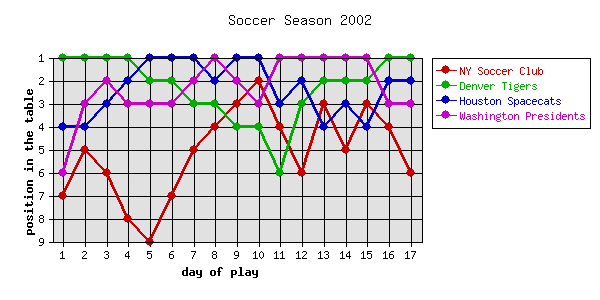
\includegraphics[scale=0.6]{d_linesp2.png}
  \end{center}
  \caption{Linespoints chart}
  \label{fig:d_linesp2}
\end{figure}
\begin{verbatim}
use Chart::LinesPoints;
use strict;

my (@data1, @data2, @data4, @data3, @labels, %hash, $g);

@labels = qw(1 2 3 4 5 6 7 8 9 10 11 12 13 14 15 16 17);
@data1  = qw (-7 -5 -6 -8 -9 -7 -5 -4 -3 -2 -4 -6 -3 -5 -3 -4 -6);
@data2  = qw (-1 -1 -1 -1 -2 -2 -3 -3 -4 -4 -6 -3 -2 -2 -2 -1 -1);
@data3  = qw (-4 -4 -3 -2 -1 -1 -1 -2 -1 -1 -3 -2 -4 -3 -4 -2 -2);
@data4  = qw (-6 -3 -2 -3 -3 -3 -2 -1 -2 -3 -1 -1 -1 -1 -1 -3 -3);

$g = Chart::LinesPoints->new(600,300);
$g->add_dataset(@labels);
$g->add_dataset(@data1);
$g->add_dataset(@data2);
$g->add_dataset(@data3);
$g->add_dataset(@data4);

%hash = ('integer_ticks_only' => 'true',
         'title'         => 'Soccer Season 2002\n ',
         'legend_labels' => ['NY Soccer Club', 'Denver Tigers',
                             'Houston Spacecats',
                             'Washington Presidents'],
         'y_label'       => 'position in the table',
         'x_label'       => 'day of play',
         'grid_lines'    => 'true',
         'f_y_tick'      => \&formatter,
        );

$g->set( %hash);

$g->png("d_linesp2.png");

# Just a trick to have the y scale start at the biggest point:
# Initialise with negative values, remove the minus sign!
sub formatter {
  my $label = shift;
  $label    = substr($label, 1);
  return $label;
}

\end{verbatim}

\constructorblurb{\thisname}

\begin{AttrDecl}{brush\_size}
Sets the width of the lines in pixels. Default is 6.
\end{AttrDecl}

\begin{AttrDecl}{brushStyle}
Define the share of the points. The share may be specified to each dataset.\\
The possible shapes of the 'points' are
\begin{itemize}
\item FilledCircle (default),
\item circle,
\item donut,
\item OpenCircle,
\item triangle,
\item upsidedownTriangle,
\item square,
\item hollowSquare,
\item OpenRectangle,
\item fatPlus,
\item Star,
\item OpenStar,
\item FilledDiamond, 
\item OpenDiamond
\end{itemize} 
To apply a different brush style to different data sets the following
example of code can be used:
\begin{verbatim}
$g->set(brushStyles => { dataset0 => 'fatPlus', dataset1 => 'hollowSquare' });
\end{verbatim}
\end{AttrDecl}


\begin{AttrDecl}{pt\_size}
Sets the radius of the points in pixels. Default is 18.
\end{AttrDecl}

\begin{AttrDecl}{sort}
Sorts the data in ascending order if set to \literal{true}. Should be
set if the input data is not sorted. Defaults to \literal{false}.
\end{AttrDecl}

\begin{AttrDecl}{stepline}
The points are connected by a stepping function,instead of by a direct
line if set to \literal{true}. Defaults to \literal{false}.
\end{AttrDecl}

\begin{AttrDecl}{stepline\_mode}
Determines whether to plot each stepping line at the level of the
start of the interval (if set to \literal{begin}) or at its end if set
to \literal{end}. Defaults to \literal{begin}.
\end{AttrDecl}

\attrdecl{xlabels}
\begin{AttrDecl}{xrange}
This pair of options allows arbitrary positioning of $x$ axis labels.
The two options must either both be specified or both be omitted.
\attruse{xlabels} is a reference to 2-element array. The first of the
elements is a nested (reference to an) array of strings that are the
labels. The second element is a nested (reference to an) array of
numbers that are the $x$ values at which the labels should be placed.
\attruse{xrange} is a 2-element array specifying the minimum and maximum
$x$ values on the axis. \Eg,
\begin{verbatim}
@labels = (['Jan', 'Feb', 'Mar'],
           [10,    40,    70   ]);
$chart->set(xlabels => \bs @labels,
            xrange  => [0, 100]
           );
\end{verbatim}
\end{AttrDecl}

\begin{AttrDecl}{xy\_plot}
Forces \thisclass to plot a $x$--$y$ graph if set to \literal{true}, \ie, to
treat the $x$ axis as numeric. Very useful for plots of mathematical
functions. Defaults to \literal{false}.
\end{AttrDecl}

\begin{AttrDecl}{y\_axes}
Tells \thisclass where to place the $y$ axis. Valid
values are \literal{left}, \literal{right} and \literal{both}. Defaults
to \literal{left}.
\end{AttrDecl}


%
% mountain.tex
%
\renewcommand{\thisname}{Chart::Mountain}
\section{\thisname}
\name{\thisname}
\file{Mountain.pm}
\requires{Chart::Base, GD, Carp, FileHandle}
\begin{Description}
The class \thisclass creates a mountain chart, \ie, the individual data
sets are stacked and the areas under the curves are colour filled.
The first data set will be shown at the top of the stack, the last at
the bottom. \thisclass is a subclass of Chart::Base.
\end{Description}

\example
\begin{figure}[ht]
  \begin{center}
    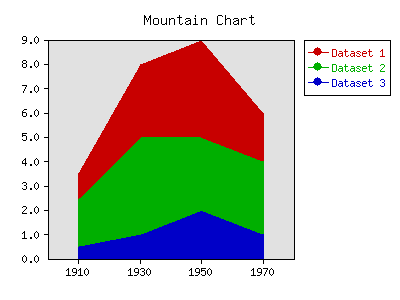
\includegraphics[scale =0.6]{mountain.png}
  \end{center}
  \caption{Mountain chart}
  \label{fig:mountain}
\end{figure}
\begin{verbatim}
use Chart::Mountain;

$g = Chart::Mountain->new();

@data = [ [1910, 1930, 1950, 1970],
          [1, 3, 4, 2],
          [2, 4, 3, 3],
          [0.5, 1, 2, 1]];

$g->set('title'      => 'Mountain Chart',
        'grid_lines' => 'false',
        'precision'  => 1);

$g->png("mountain.png", @data);
\end{verbatim}

\constructorblurb{\thisname}

\begin{AttrDecl}{y\_axes}
Tells \thisclass where to place the $y$ axis. Valid
values are \literal{left}, \literal{right} and \literal{both}. Defaults
to \literal{left}.
\end{AttrDecl}

%
% pareto.tex
%
\renewcommand{\thisname}{Chart::Pareto}
\section{\thisname}
\name{\thisname}
\file{Pareto.pm}
\requires{Chart::Base, GD, Carp, FileHandle}
\begin{Description}
The class \thisclass creates a Pareto chart, \ie, a set of absolute
values overlaid with a line chart of the accumulated values. (This
latter curve is also known as an \emph{empirical cumulative distribution
function} or as a \emph{Lorenz curve}.) This representation usually
makes sense only if the values are sorted (either in ascending or in
descending order). \thisclass plots only one data set and its labels.
\thisclass is a subclass of \class{Chart::Base}.
\end{Description}

\example

\begin{figure}[ht]
  \begin{center}
    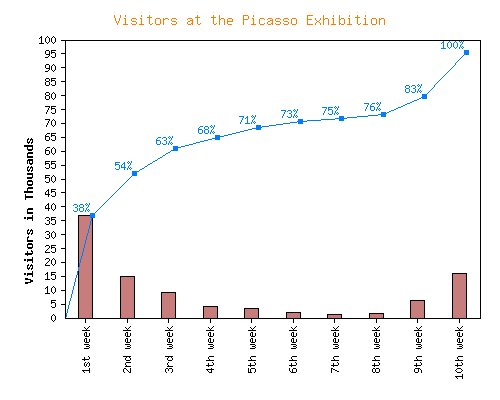
\includegraphics[scale=0.7]{d_pareto2.png}
  \end{center}
  \caption{Pareto chart}
  \label{fig:pareto}
\end{figure}
\begin{verbatim}
use Chart::Pareto;

$g = Chart::Pareto->new(500,400);
$g->add_dataset('1st week', '2nd week', '3rd week', '4th week',
                '5th week', '6th week', '7th week', '8th week',
                '9th week', '10th week');
$g->add_dataset(37, 15, 9, 4, 3.5, 2.1, 1.2, 1.5, 6.2, 16);

%hash = ('colors' => { 'dataset0' => 'mauve',
                       'dataset1' => 'light_blue',
                       'title' => 'orange'
                     },
         'title'              => 'Visitors at the Picasso Exhibition',
         'integer_ticks_only' => 'true',
         'skip_int_ticks'     => 5,
         'grey_background'    => 'false',
         'max_val'            => 100,
         'y_label'            => 'Visitors in Thousands',
         'x_ticks'            => 'vertical',
         'spaced_bars'        => 'true',
         'legend'             => 'none'
        );

$g->set(%hash);

$g->png("pareto.png");
\end{verbatim}

\constructorblurb{\thisname}

\begin{AttrDecl}{sort}
Sorts the data in ascending order if set to \literal{true}. Should be set if
the input data is not sorted. Defaults to \literal{false}.
\end{AttrDecl}

\begin{AttrDecl}{spaced\_bars}
Leaves some space between each group of bars when set to \literal{true}. This
usually make it easier to read a bar chart. Default is \literal{true}.
\end{AttrDecl}

\begin{AttrDecl}{y\_axes}
Tells \thisclass where to place the $y$ axis. Valid
values are \literal{left}, \literal{right} and \literal{both}. Defaults
to \literal{left}.
\end{AttrDecl}

%
% pie.tex
%
\renewcommand{\thisname}{Chart::Pie}
\section{\thisname}
\name{\thisname}
\file{Pie.pm}
\requires{Chart::Base, GD, Carp, FileHandle}
\begin{Description}
The class \thisclass creates a pie chart. The first added set must
contain the labels, the second set the values. \thisclass is a subclass
of \class{Chart::Base}.
\end{Description}

\example
\begin{figure}[ht]
  \begin{center}
    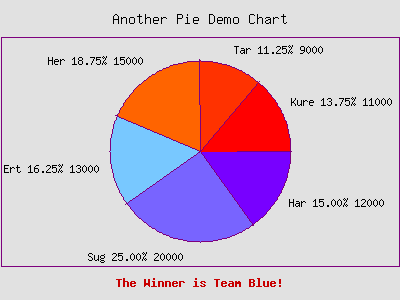
\includegraphics[scale = 0.6]{d_pie3.png}
  \end{center}
  \caption{Pie chart}
  \label{fig:pie}
\end{figure}
\begin{verbatim}
use Chart::Pie;

$g = Chart::Pie->new();

$g->add_dataset('Har', 'Sug', 'Ert', 'Her', 'Tar', 'Kure');
$g->add_dataset(12000, 20000 , 13000, 15000, 9000, 11000  );

%opt = ('title'        => 'Another Pie Demo Chart',
        'label_values' => 'both',
        'legend'       => 'none',
        'text_space'   => 10,
        'png_border'   => 1,
        'graph_border' => 0,
        'colors' => { 'x_label'    => 'red',
                      'misc'       => 'plum',
                      'background' => 'grey',
                      'dataset0'   => [120, 0, 255],
                      'dataset1'   => [120, 100, 255],
                      'dataset2'   => [120, 200, 255],
                      'dataset3'   => [255, 100, 0],
                      'dataset4'   => [255, 50, 0],
                      'dataset5'   => [255, 0, 0],
                    },
        'x_label'      => 'The Winner is Team Blue!',
       );

$g->set(%opt);

$g->png("pie.png");
\end{verbatim}

\constructorblurb{\thisname}

\begin{AttrDecl}{label\_values}
Tells \thisclass what kind of value labels to show alongside the pie.
Valid values are \literal{percent}, \literal{value}, \literal{both} and
\literal{none}. Defaults to \literal{percent}.
\end{AttrDecl}

\begin{AttrDecl}{legend\_label\_values}
Tells \thisclass what kind of labels to show in the legend. Valid values
are \literal{percent}, \literal{value}, \literal{both} and
\literal{none}. Defaults to \literal{value}.
\end{AttrDecl}

\begin{AttrDecl}{legend\_lines}
The labels drawn alongside the pie are connected with a line to the
segment if this option is set to \literal{true}.
\end{AttrDecl}

\begin{AttrDecl}{ring}
The pie can have a ring shape instead of the usual disc shape. This
option determines the thickness of the ring as a fraction of the radius.
Default is 1, \ie, a full pie.
\end{AttrDecl}

%
% points.tex
%
\renewcommand{\thisname}{Chart::Points}
\section{\thisname}
\name{\thisname}
\file{Points.pm}
\requires{Chart::Base, GD, Carp, FileHandle}
\begin{Description}
The class \thisclass creates a point chart (also called
\emph{scattergram}) where the individual data points are marked with a
symbol. (If you want lines in addition, check
\class{Chart::LinesPoints} on page~\pageref{Chart::LinesPoints}.)
\thisclass is a subclass of \class{Chart::Base}.
\end{Description}

\example
\begin{figure}[ht]
  \begin{center}
    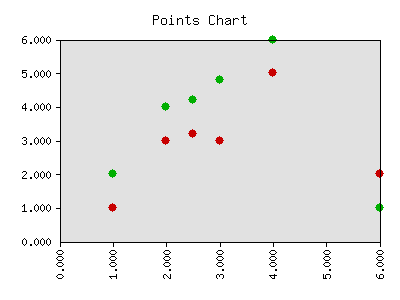
\includegraphics[scale=0.5]{points.png}
  \end{center}
  \caption{Points chart}
  \label{fig:points}
\end{figure}

\begin{verbatim}
use Chart::Points;

$g = Chart::Points->new();
$g->add_dataset(1, 4,   3, 6, 2, 2.5);  # x-coordinates
$g->add_dataset(1, 5,   3, 2, 3, 3.2);  # y-coordinates dataset 1
$g->add_dataset(2, 6, 4.8, 1, 4, 4.2);  # y-coordinates dataset 2

@hash = ('title'        => 'Points Chart',
         'xy_plot'      => 'true',
         'x_ticks'      => 'vertical',
         'legend'       => 'none',
         'sort'         => 'true',
         'precision'    => 3,
         'include_zero' => 'true',
        );

$g->set(@hash);

$g->png("Grafiken/points.png");
\end{verbatim}

\constructorblurb{\thisname}

\begin{AttrDecl}{pt\_size}
Sets the radius of the points in pixels. Default is 18.\\
The points are extended by different brush styles.
\end{AttrDecl}

\begin{AttrDecl}{brushStyle}
Define the share of the points. The share may be specified to each dataset.\\
The possible shapes of the 'points' are
\begin{itemize}
\item FilledCircle (default),
\item circle,
\item donut,
\item OpenCircle,
\item triangle,
\item upsidedownTriangle,
\item square,
\item hollowSquare,
\item OpenRectangle,
\item fatPlus,
\item Star,
\item OpenStar,
\item FilledDiamond, 
\item OpenDiamond
\end{itemize} 
To apply a different brush style to different data sets the following
example of code can be used:
\begin{verbatim}
$g->set(brushStyles => { dataset0 => 'fatPlus', dataset1 => 'hollowSquare' });
\end{verbatim}
\begin{figure}[htp]
  \begin{center}
    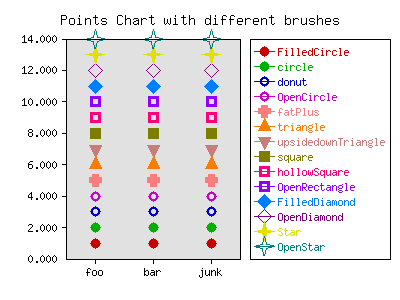
\includegraphics{brushstyles.png}
  \end{center}
  \caption{Points chart as an example for brush styles}
  \label{fig:brushStyles}
\end{figure}
\end{AttrDecl}

\begin{AttrDecl}{sort}
Sorts the data in ascending order if set to \literal{true}. Should be
set if the input data is not sorted. Defaults to \literal{false}.
\end{AttrDecl}

\attrdecl{xlabels}
\begin{AttrDecl}{xrange}
This pair of options allows arbitrary positioning of $x$ axis labels.
The two options must either both be specified or both be omitted.
\attruse{xlabels} is a reference to 2-element array. The first of the
elements is a nested (reference to an) array of strings that are the
labels. The second element is a nested (reference to an) array of
numbers that are the $x$ values at which the labels should be placed.
\attruse{xrange} is a 2-element array specifying the minimum and maximum
$x$ values on the axis. \Eg,
\begin{verbatim}
@labels = (['Jan', 'Feb', 'Mar'],
           [10,    40,    70   ]);
$chart->set(xlabels => \bs @labels,
            xrange  => [0, 100]
           );
\end{verbatim}
\end{AttrDecl}

\begin{AttrDecl}{xy\_plot}
Forces \thisclass to plot a $x$--$y$ graph if set to \literal{true},
\ie, to treat the $x$ axis as numeric. Very useful for plots of
mathematical functions. Defaults to \literal{false}.
\end{AttrDecl}

\begin{AttrDecl}{y\_axes}
Tells \thisclass where to place the $y$ axis. Valid
values are \literal{left}, \literal{right} and \literal{both}. Defaults
to \literal{left}.
\end{AttrDecl}

%
% split.tex
%
\renewcommand{\thisname}{Chart::Split}
\section{\thisname}
\name{\thisname}
\file{Split.pm}
\requires{Chart::Base, GD, Carp, FileHandle}
\begin{Description}
The class \thisclass creates a lines chart where both $x$ and $y$ axes
are assumed to be numeric. Split charts are mainly intended for cases
where many data points are spread over a wide $x$ range while at the
same time the $y$ range is limited. Typical examples are weather or
seismic data. The $x$ axis will be split into several intervals of the
same length (specified with the mandatory option \attruse{interval}).
The intervals will be displayed in a stacked fashion. The start of the
top interval is set with the mandatory option \attruse{start}.
\thisclass will draw only positive $x$ coordinates. The $y$ axis will
not be labelled with the $y$ values. Rather, the axis will show only
the sequence numbers of the intervals. \thisclass is a subclass of
\class{Chart::Base}.
\end{Description}

\example

\begin{figure}[ht]
  \begin{center}
    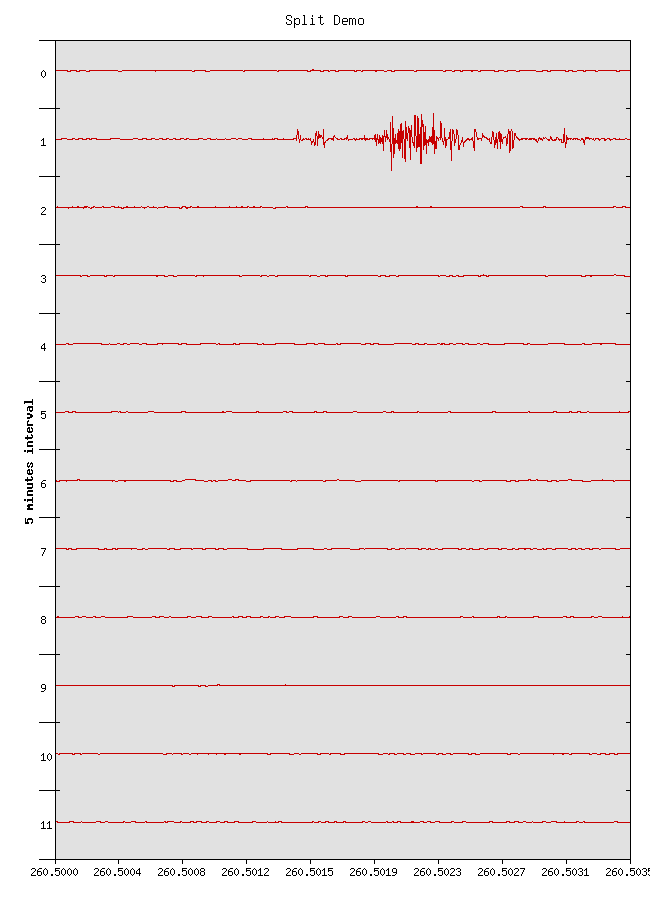
\includegraphics[width=\textwidth, height=\textwidth]{stunde.png}
  \end{center}
  \caption{Split chart}
  \label{fig:split}
\end{figure}
\begin{verbatim}
use Chart::Split;

$g = Chart::Split->new(650, 900);

# Get the data from a file and push them into arrays
open(FILE, "data.dat") or die "Can't open the data file!\n";
while (<FILE>) {
  ($x, $y) = split;
   push (@x, $x);
   push (@y, $y);
}
close(FILE);

# Add the data
$g->add_dataset(@x);
$g->add_dataset(@y);

# Set the options
$g->set('xy_plot'        => 'true');
$g->set('legend'         => 'none');
$g->set('title'          => 'Split Demo');
$g->set('interval'       => 1/288);
$g->set('interval_ticks' => 10);
$g->set('start'          => 260.5);
$g->set('brush_size'     => 1);
$g->set('precision'      => 4);
$g->set('y_label'        => '5 minutes interval');

# Give me a nice picture
$g->png("split.png");
\end{verbatim}

\constructorblurb{\thisname}

\begin{AttrDecl}{start}
Sets the start value of the first interval. If the $x$ coordinate of
the first data point is 0, \attruse{start} should also be set to 0.
\emph{Required} value for a \thisclass chart. Defaults to undef.
\end{AttrDecl}

\begin{AttrDecl}{interval}
Sets the interval of one segment to plot. \emph{Required} value for a
split chart. Defaults to undef.
\end{AttrDecl}

\begin{AttrDecl}{interval\_ticks}
Sets the number of ticks for the $x$ axis. Defaults to 5.
\end{AttrDecl}

\begin{AttrDecl}{scale}
Every $y$ value of a \thisclass chart will be multiplied by this value,
without however changing the sclaing of the $y$ axis. (This might result
in some segments being overdrawn by others.) Only useful if you want to
give prominence to the maximal amplitudes of data. Defaults to 1.
\end{AttrDecl}

\begin{AttrDecl}{sort}
Sorts the data in ascending order if set to \literal{true}. Should be set if
the input data is not sorted. Defaults to \literal{false}.
\end{AttrDecl}

\begin{AttrDecl}{y\_axes}
Tells \thisclass where to place the $y$ axis. Valid
values are \literal{left}, \literal{right} and \literal{both}. Defaults
to \literal{left}.
\end{AttrDecl}

%
% stacked.tex
%
\renewcommand{\thisname}{Chart::StackedBars}
\section{\thisname}
\name{\thisname}
\file{StackedBars.pm}
\requires{Chart::Base, GD, Carp, FileHandle}
\begin{Description}
The class \thisclass creates a chart made up of stacked vertical bars.
The first data set will be shown at the bottom of the stack, the last at
the top. \thisclass is a subclass of \class{Chart::Base}.
\end{Description}

\example
\begin{figure}[ht]
  \begin{center}
    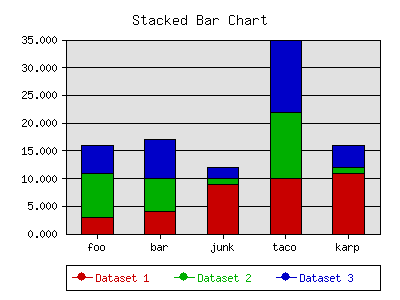
\includegraphics[scale=0.6]{stackedbars.png}
  \end{center}
  \caption{Chart with stacked bars}
  \label{fig:stackedbars}
\end{figure}
\begin{verbatim}
use Chart::StackedBars;

$g = Chart::StackedBars->new();

$g->add_dataset(qw(foo bar junk taco karp));
$g->add_dataset(3, 4, 9, 10, 11);
$g->add_dataset(8, 6, 1, 12, 1);
$g->add_dataset(5, 7, 2, 13, 4);

$g->set('title'        => 'Stacked Bar Chart');
$g->set('y_grid_lines' => 'true');
$g->set('legend'       => 'bottom');

$g->png("stackedbars.png");
\end{verbatim}

\constructorblurb{\thisname}

\begin{AttrDecl}{spaced\_bars}
Leaves some space between the individual bars when set to
\literal{true}. This usually make it easier to read a bar chart, with
stacked bars, however, it is not as important as with groups of bars.
Default is \literal{true}.
\end{AttrDecl}

\begin{AttrDecl}{y\_axes}
Tells \thisclass where to place the $y$ axis. Valid values are
\literal{left}, \literal{right} and \literal{both}. Defaults to
\literal{left}.
\end{AttrDecl}

%\include{Colors}
%
% Appendix.tex
%
\section{Appendix}
\renewcommand{\thisname}{Named Colors}
\name{\thisname}
\label{app:colors}

The following list summarizes the named colors which can be defined in respect to \textsc{rgb} 
values. The colors are defined by\\
\methoduse{\$obj->set('colors' \fatcomma \{'background' \fatcomma 'green'\});}

\vspace{2ex}
%
% AppendixRGB.tex
%

The list of all defined colors is:\\ 
white
black
red
green
blue
orange
orange2
orange3
orange4
yellow
purple
light\_blue
light\_green
light\_purple
pink
peach
olive
plum
turquoise
mauve
brown
grey
HotPink
PaleGreen1
PaleGreen2
PaleGreen3
PaleGreen4
DarkBlue
BlueViolet
PeachPuff
PeachPuff1
PeachPuff2
PeachPuff3
PeachPuff4
chocolate1
chocolate2
chocolate3
chocolate4
LightGreen
lavender
MediumPurple
DarkOrange
DarkOrange2
DarkOrange3
DarkOrange4
SlateBlue
BlueViolet
RoyalBlue
AntiqueWhite
AntiqueWhite1
AntiqueWhite2
AntiqueWhite3
AntiqueWhite4
CadetBlue
CadetBlue1
CadetBlue2
CadetBlue3
CadetBlue4
DarkGoldenrod
DarkGoldenrod1
DarkGoldenrod2
DarkGoldenrod3
DarkGoldenrod4
DarkOliveGreen
DarkOliveGreen1
DarkOliveGreen2
DarkOliveGreen3
DarkOliveGreen4
DarkOrange1
DarkOrchid
DarkOrchid1
DarkOrchid2
DarkOrchid3
DarkOrchid4
DarkSeaGreen
DarkSeaGreen1
DarkSeaGreen2
DarkSeaGreen3
DarkSeaGreen4
DarkSlateGray
DarkSlateGray1
DarkSlateGray2
DarkSlateGray3
DarkSlateGray4
DeepPink
DeepPink1
DeepPink2
DeepPink3
DeepPink4
DeepSkyBlue
DeepSkyBlue1
DeepSkyBlue2
DeepSkyBlue3
DeepSkyBlue4
DodgerBlue
DodgerBlue1
DodgerBlue2
DodgerBlue3
DodgerBlue4
HotPink1
HotPink2
HotPink3
HotPink4
IndianRed
IndianRed1
IndianRed2
IndianRed3
IndianRed4
LavenderBlush
LavenderBlush1
LavenderBlush2
LavenderBlush3
LavenderBlush4
LemonChiffon
LemonChiffon1
LemonChiffon2
LemonChiffon3
LemonChiffon4
LightBlue
LightBlue1
LightBlue2
LightBlue3
LightBlue4
LightCyan
LightCyan1
LightCyan2
LightCyan3
LightCyan4
LightGoldenrod
LightGoldenrod1
LightGoldenrod2
LightGoldenrod3
LightGoldenrod4
LightPink
LightPink1
LightPink2
LightPink3
LightPink4
LightSalmon
LightSalmon1
LightSalmon2
LightSalmon3
LightSalmon4
LightSkyBlue
LightSkyBlue1
LightSkyBlue2
LightSkyBlue3
LightSkyBlue4
LightSteelBlue
LightSteelBlue1
LightSteelBlue2
LightSteelBlue3
LightSteelBlue4
LightYellow
LightYellow1
LightYellow2
LightYellow3
LightYellow4
MediumOrchid
MediumOrchid1
MediumOrchid2
MediumOrchid3
MediumOrchid4
MediumPurple1
MediumPurple2
MediumPurple3
MediumPurple4
MistyRose
MistyRose1
MistyRose2
MistyRose3
MistyRose4
NavajoWhite
NavajoWhite1
NavajoWhite2
NavajoWhite3
NavajoWhite4
OliveDrab
OliveDrab1
OliveDrab2
OliveDrab3
OliveDrab4
OrangeRed
OrangeRed1
OrangeRed2
OrangeRed3
OrangeRed4
PaleGreen
PaleTurquoise
PaleTurquoise1
PaleTurquoise2
PaleTurquoise3
PaleTurquoise4
PaleVioletRed
PaleVioletRed1
PaleVioletRed2
PaleVioletRed3
PaleVioletRed4
RosyBrown
RosyBrown1
RosyBrown2
RosyBrown3
RosyBrown4
RoyalBlue1
RoyalBlue2
RoyalBlue3
RoyalBlue4
SeaGreen
SeaGreen1
SeaGreen2
SeaGreen3
SeaGreen4
SkyBlue
SkyBlue1
SkyBlue2
SkyBlue3
SkyBlue4
SlateBlue1
SlateBlue2
SlateBlue3
SlateBlue4
SlateGray
SlateGray1
SlateGray2
SlateGray3
SlateGray4
SpringGreen
SpringGreen1
SpringGreen2
SpringGreen3
SpringGreen4
SteelBlue
SteelBlue1
SteelBlue2
SteelBlue3
SteelBlue4
VioletRed
VioletRed1
VioletRed2
VioletRed3
VioletRed4
aquamarine
aquamarine1
aquamarine2
aquamarine3
aquamarine4
azure
azure1
azure2
azure3
azure4
bisque
bisque1
bisque2
bisque3
bisque4
blue1
blue2
blue3
blue4
brown1
brown2
brown3
brown4
burlywood
burlywood1
burlywood2
burlywood3
burlywood4
chartreuse
chartreuse1
chartreuse2
chartreuse3
chartreuse4
chocolate
coral
coral1
coral2
coral3
coral4
cornsilk
cornsilk1
cornsilk2
cornsilk3
cornsilk4
cyan
cyan1
cyan2
cyan3
cyan4
firebrick
firebrick1
firebrick2
firebrick3
firebrick4
gold
gold1
gold2
gold3
gold4
goldenrod
goldenrod1
goldenrod2
goldenrod3
goldenrod4
gray
gray1
gray2
gray3
gray4
green1
green2
green3
green4
grey1
grey2
grey3
grey4
honeydew
honeydew1
honeydew2
honeydew3
honeydew4
ivory
ivory1
ivory2
ivory3
ivory4
khaki
khaki1
khaki2
khaki3
khaki4
magenta
magenta1
magenta2
magenta3
magenta4
maroon
maroon1
maroon2
maroon3
maroon4
orange1
orchid
orchid1
orchid2
orchid3
orchid4
pink1
pink2
pink3
pink4
plum1
plum2
plum3
plum4
purple1
purple2
purple3
purple4
red1
red2
red3
red4
salmon
salmon1
salmon2
salmon3
salmon4
seashell
seashell1
seashell2
seashell3
seashell4
sienna
sienna1
sienna2
sienna3
sienna4
snow
snow1
snow2
snow3
snow4
tan
tan1
tan2
tan3
tan4
thistle
thistle1
thistle2
thistle3
thistle4
tomato
tomato1
tomato2
tomato3
tomato4
turquoise1
turquoise2
turquoise3
turquoise4
wheat
wheat1
wheat2
wheat3
wheat4
yellow1
yellow2
yellow3
yellow4


\vspace{2ex}
The following tables will show the named colors, the corresponding RGB values and an example of the colors.


\begin{tabular}{|l|c|c|}
white & [ 255, 255, 255 ] & \color{white} \rule{1cm}{1.5ex}\\
black & [ 0, 0, 0 ] & \color{black} \rule{1cm}{1.5ex}\\
red & [ 200, 0, 0 ] & \color{red} \rule{1cm}{1.5ex}\\
green & [ 0, 175, 0 ] & \color{green} \rule{1cm}{1.5ex}\\
blue & [ 0, 0, 200 ] & \color{blue} \rule{1cm}{1.5ex}\\
orange & [ 250, 125, 0 ] & \color{orange} \rule{1cm}{1.5ex}\\
orange2 & [ 238, 154, 0 ] & \color{orange2} \rule{1cm}{1.5ex}\\
orange3 & [ 205, 133, 0 ] & \color{orange3} \rule{1cm}{1.5ex}\\
orange4 & [ 139, 90, 0 ] & \color{orange4} \rule{1cm}{1.5ex}\\
yellow & [ 225, 225, 0 ] & \color{yellow} \rule{1cm}{1.5ex}\\
purple & [ 200, 0, 200 ] & \color{purple} \rule{1cm}{1.5ex}\\
light\_blue & [ 0, 125, 250 ] & \color{light_blue} \rule{1cm}{1.5ex}\\
light\_green & [ 125, 250, 0 ] & \color{light_green} \rule{1cm}{1.5ex}\\
light\_purple & [ 145, 0, 250 ] & \color{light_purple} \rule{1cm}{1.5ex}\\
pink & [ 250, 0, 125 ] & \color{pink} \rule{1cm}{1.5ex}\\
peach & [ 250, 125, 125 ] & \color{peach} \rule{1cm}{1.5ex}\\
olive & [ 125, 125, 0 ] & \color{olive} \rule{1cm}{1.5ex}\\
plum & [ 125, 0, 125 ] & \color{plum} \rule{1cm}{1.5ex}\\
turquoise & [ 0, 125, 125 ] & \color{turquoise} \rule{1cm}{1.5ex}\\
mauve & [ 200, 125, 125 ] & \color{mauve} \rule{1cm}{1.5ex}\\
brown & [ 160, 80, 0 ] & \color{brown} \rule{1cm}{1.5ex}\\
grey & [ 225, 225, 225 ] & \color{grey} \rule{1cm}{1.5ex}\\
HotPink & [ 255, 105, 180 ] & \color{HotPink} \rule{1cm}{1.5ex}\\
PaleGreen1 & [ 154, 255, 154 ] & \color{PaleGreen1} \rule{1cm}{1.5ex}\\
PaleGreen2 & [ 144, 238, 144 ] & \color{PaleGreen2} \rule{1cm}{1.5ex}\\
PaleGreen3 & [ 124, 205, 124 ] & \color{PaleGreen3} \rule{1cm}{1.5ex}\\
PaleGreen4 & [ 84, 138, 84 ] & \color{PaleGreen4} \rule{1cm}{1.5ex}\\
DarkBlue & [ 0, 0, 139 ] & \color{DarkBlue} \rule{1cm}{1.5ex}\\
BlueViolet & [ 138, 43, 226 ] & \color{BlueViolet} \rule{1cm}{1.5ex}\\
PeachPuff & [ 255, 218, 185 ] & \color{PeachPuff} \rule{1cm}{1.5ex}\\
PeachPuff1 & [ 255, 218, 185 ] & \color{PeachPuff1} \rule{1cm}{1.5ex}\\
PeachPuff2 & [ 238, 203, 173 ] & \color{PeachPuff2} \rule{1cm}{1.5ex}\\
PeachPuff3 & [ 205, 175, 149 ] & \color{PeachPuff3} \rule{1cm}{1.5ex}\\
PeachPuff4 & [ 139, 119, 101 ] & \color{PeachPuff4} \rule{1cm}{1.5ex}\\
chocolate1 & [ 255, 127, 36 ] & \color{chocolate1} \rule{1cm}{1.5ex}\\
chocolate2 & [ 238, 118, 33 ] & \color{chocolate2} \rule{1cm}{1.5ex}\\
chocolate3 & [ 205, 102, 29 ] & \color{chocolate3} \rule{1cm}{1.5ex}\\
chocolate4 & [ 139, 69, 19 ] & \color{chocolate4} \rule{1cm}{1.5ex}\\
LightGreen & [ 144, 238, 144 ] & \color{LightGreen} \rule{1cm}{1.5ex}\\
\end{tabular}


\begin{tabular}{|l|c|c|}
lavender & [ 230, 230, 250 ] & \color{lavender} \rule{1cm}{1.5ex}\\
MediumPurple & [ 147, 112, 219 ] & \color{MediumPurple} \rule{1cm}{1.5ex}\\
DarkOrange & [ 255, 127, 0 ] & \color{DarkOrange} \rule{1cm}{1.5ex}\\
DarkOrange2 & [ 238, 118, 0 ] & \color{DarkOrange2} \rule{1cm}{1.5ex}\\
DarkOrange3 & [ 205, 102, 0 ] & \color{DarkOrange3} \rule{1cm}{1.5ex}\\
DarkOrange4 & [ 139, 69, 0 ] & \color{DarkOrange4} \rule{1cm}{1.5ex}\\
SlateBlue & [ 106, 90, 205 ] & \color{SlateBlue} \rule{1cm}{1.5ex}\\
BlueViolet & [ 138, 43, 226 ] & \color{BlueViolet} \rule{1cm}{1.5ex}\\
RoyalBlue & [ 65, 105, 225 ] & \color{RoyalBlue} \rule{1cm}{1.5ex}\\
AntiqueWhite & [ 250, 235, 215 ] & \color{AntiqueWhite} \rule{1cm}{1.5ex}\\
AntiqueWhite1 & [ 255, 239, 219 ] & \color{AntiqueWhite1} \rule{1cm}{1.5ex}\\
AntiqueWhite2 & [ 238, 223, 204 ] & \color{AntiqueWhite2} \rule{1cm}{1.5ex}\\
AntiqueWhite3 & [ 205, 192, 176 ] & \color{AntiqueWhite3} \rule{1cm}{1.5ex}\\
AntiqueWhite4 & [ 139, 131, 120 ] & \color{AntiqueWhite4} \rule{1cm}{1.5ex}\\
CadetBlue & [ 95, 158, 160 ] & \color{CadetBlue} \rule{1cm}{1.5ex}\\
CadetBlue1 & [ 152, 245, 255 ] & \color{CadetBlue1} \rule{1cm}{1.5ex}\\
CadetBlue2 & [ 142, 229, 238 ] & \color{CadetBlue2} \rule{1cm}{1.5ex}\\
CadetBlue3 & [ 122, 197, 205 ] & \color{CadetBlue3} \rule{1cm}{1.5ex}\\
CadetBlue4 & [ 83, 134, 139 ] & \color{CadetBlue4} \rule{1cm}{1.5ex}\\
DarkGoldenrod & [ 184, 134, 11 ] & \color{DarkGoldenrod} \rule{1cm}{1.5ex}\\
DarkGoldenrod1 & [ 255, 185, 15 ] & \color{DarkGoldenrod1} \rule{1cm}{1.5ex}\\
DarkGoldenrod2 & [ 238, 173, 14 ] & \color{DarkGoldenrod2} \rule{1cm}{1.5ex}\\
DarkGoldenrod3 & [ 205, 149, 12 ] & \color{DarkGoldenrod3} \rule{1cm}{1.5ex}\\
DarkGoldenrod4 & [ 139, 101, 8 ] & \color{DarkGoldenrod4} \rule{1cm}{1.5ex}\\
DarkOliveGreen & [ 85, 107, 47 ] & \color{DarkOliveGreen} \rule{1cm}{1.5ex}\\
DarkOliveGreen1 & [ 202, 255, 112 ] & \color{DarkOliveGreen1} \rule{1cm}{1.5ex}\\
DarkOliveGreen2 & [ 188, 238, 104 ] & \color{DarkOliveGreen2} \rule{1cm}{1.5ex}\\
DarkOliveGreen3 & [ 162, 205, 90 ] & \color{DarkOliveGreen3} \rule{1cm}{1.5ex}\\
DarkOliveGreen4 & [ 110, 139, 61 ] & \color{DarkOliveGreen4} \rule{1cm}{1.5ex}\\
DarkOrange1 & [ 255, 127, 0 ] & \color{DarkOrange1} \rule{1cm}{1.5ex}\\
DarkOrchid & [ 153, 50, 204 ] & \color{DarkOrchid} \rule{1cm}{1.5ex}\\
DarkOrchid1 & [ 191, 62, 255 ] & \color{DarkOrchid1} \rule{1cm}{1.5ex}\\
DarkOrchid2 & [ 178, 58, 238 ] & \color{DarkOrchid2} \rule{1cm}{1.5ex}\\
DarkOrchid3 & [ 154, 50, 205 ] & \color{DarkOrchid3} \rule{1cm}{1.5ex}\\
DarkOrchid4 & [ 104, 34, 139 ] & \color{DarkOrchid4} \rule{1cm}{1.5ex}\\
DarkSeaGreen & [ 143, 188, 143 ] & \color{DarkSeaGreen} \rule{1cm}{1.5ex}\\
DarkSeaGreen1 & [ 193, 255, 193 ] & \color{DarkSeaGreen1} \rule{1cm}{1.5ex}\\
DarkSeaGreen2 & [ 180, 238, 180 ] & \color{DarkSeaGreen2} \rule{1cm}{1.5ex}\\
DarkSeaGreen3 & [ 155, 205, 155 ] & \color{DarkSeaGreen3} \rule{1cm}{1.5ex}\\
\end{tabular}


\begin{tabular}{|l|c|c|}
DarkSeaGreen4 & [ 105, 139, 105 ] & \color{DarkSeaGreen4} \rule{1cm}{1.5ex}\\
DarkSlateGray & [ 47, 79, 79 ] & \color{DarkSlateGray} \rule{1cm}{1.5ex}\\
DarkSlateGray1 & [ 151, 255, 255 ] & \color{DarkSlateGray1} \rule{1cm}{1.5ex}\\
DarkSlateGray2 & [ 141, 238, 238 ] & \color{DarkSlateGray2} \rule{1cm}{1.5ex}\\
DarkSlateGray3 & [ 121, 205, 205 ] & \color{DarkSlateGray3} \rule{1cm}{1.5ex}\\
DarkSlateGray4 & [ 82, 139, 139 ] & \color{DarkSlateGray4} \rule{1cm}{1.5ex}\\
DeepPink & [ 255, 20, 147 ] & \color{DeepPink} \rule{1cm}{1.5ex}\\
DeepPink1 & [ 255, 20, 147 ] & \color{DeepPink1} \rule{1cm}{1.5ex}\\
DeepPink2 & [ 238, 18, 137 ] & \color{DeepPink2} \rule{1cm}{1.5ex}\\
DeepPink3 & [ 205, 16, 118 ] & \color{DeepPink3} \rule{1cm}{1.5ex}\\
DeepPink4 & [ 139, 10, 80 ] & \color{DeepPink4} \rule{1cm}{1.5ex}\\
DeepSkyBlue & [ 0, 191, 255 ] & \color{DeepSkyBlue} \rule{1cm}{1.5ex}\\
DeepSkyBlue1 & [ 0, 191, 255 ] & \color{DeepSkyBlue1} \rule{1cm}{1.5ex}\\
DeepSkyBlue2 & [ 0, 178, 238 ] & \color{DeepSkyBlue2} \rule{1cm}{1.5ex}\\
DeepSkyBlue3 & [ 0, 154, 205 ] & \color{DeepSkyBlue3} \rule{1cm}{1.5ex}\\
DeepSkyBlue4 & [ 0, 104, 139 ] & \color{DeepSkyBlue4} \rule{1cm}{1.5ex}\\
DodgerBlue & [ 30, 144, 255 ] & \color{DodgerBlue} \rule{1cm}{1.5ex}\\
DodgerBlue1 & [ 30, 144, 255 ] & \color{DodgerBlue1} \rule{1cm}{1.5ex}\\
DodgerBlue2 & [ 28, 134, 238 ] & \color{DodgerBlue2} \rule{1cm}{1.5ex}\\
DodgerBlue3 & [ 24, 116, 205 ] & \color{DodgerBlue3} \rule{1cm}{1.5ex}\\
DodgerBlue4 & [ 16, 78, 139 ] & \color{DodgerBlue4} \rule{1cm}{1.5ex}\\
HotPink1 & [ 255, 110, 180 ] & \color{HotPink1} \rule{1cm}{1.5ex}\\
HotPink2 & [ 238, 106, 167 ] & \color{HotPink2} \rule{1cm}{1.5ex}\\
HotPink3 & [ 205, 96, 144 ] & \color{HotPink3} \rule{1cm}{1.5ex}\\
HotPink4 & [ 139, 58, 98 ] & \color{HotPink4} \rule{1cm}{1.5ex}\\
IndianRed & [ 205, 92, 92 ] & \color{IndianRed} \rule{1cm}{1.5ex}\\
IndianRed1 & [ 255, 106, 106 ] & \color{IndianRed1} \rule{1cm}{1.5ex}\\
IndianRed2 & [ 238, 99, 99 ] & \color{IndianRed2} \rule{1cm}{1.5ex}\\
IndianRed3 & [ 205, 85, 85 ] & \color{IndianRed3} \rule{1cm}{1.5ex}\\
IndianRed4 & [ 139, 58, 58 ] & \color{IndianRed4} \rule{1cm}{1.5ex}\\
LavenderBlush & [ 255, 240, 245 ] & \color{LavenderBlush} \rule{1cm}{1.5ex}\\
LavenderBlush1 & [ 255, 240, 245 ] & \color{LavenderBlush1} \rule{1cm}{1.5ex}\\
LavenderBlush2 & [ 238, 224, 229 ] & \color{LavenderBlush2} \rule{1cm}{1.5ex}\\
LavenderBlush3 & [ 205, 193, 197 ] & \color{LavenderBlush3} \rule{1cm}{1.5ex}\\
LavenderBlush4 & [ 139, 131, 134 ] & \color{LavenderBlush4} \rule{1cm}{1.5ex}\\
LemonChiffon & [ 255, 250, 205 ] & \color{LemonChiffon} \rule{1cm}{1.5ex}\\
LemonChiffon1 & [ 255, 250, 205 ] & \color{LemonChiffon1} \rule{1cm}{1.5ex}\\
LemonChiffon2 & [ 238, 233, 191 ] & \color{LemonChiffon2} \rule{1cm}{1.5ex}\\
LemonChiffon3 & [ 205, 201, 165 ] & \color{LemonChiffon3} \rule{1cm}{1.5ex}\\
\end{tabular}


\begin{tabular}{|l|c|c|}
LemonChiffon4 & [ 139, 137, 112 ] & \color{LemonChiffon4} \rule{1cm}{1.5ex}\\
LightBlue & [ 173, 216, 230 ] & \color{LightBlue} \rule{1cm}{1.5ex}\\
LightBlue1 & [ 191, 239, 255 ] & \color{LightBlue1} \rule{1cm}{1.5ex}\\
LightBlue2 & [ 178, 223, 238 ] & \color{LightBlue2} \rule{1cm}{1.5ex}\\
LightBlue3 & [ 154, 192, 205 ] & \color{LightBlue3} \rule{1cm}{1.5ex}\\
LightBlue4 & [ 104, 131, 139 ] & \color{LightBlue4} \rule{1cm}{1.5ex}\\
LightCyan & [ 224, 255, 255 ] & \color{LightCyan} \rule{1cm}{1.5ex}\\
LightCyan1 & [ 224, 255, 255 ] & \color{LightCyan1} \rule{1cm}{1.5ex}\\
LightCyan2 & [ 209, 238, 238 ] & \color{LightCyan2} \rule{1cm}{1.5ex}\\
LightCyan3 & [ 180, 205, 205 ] & \color{LightCyan3} \rule{1cm}{1.5ex}\\
LightCyan4 & [ 122, 139, 139 ] & \color{LightCyan4} \rule{1cm}{1.5ex}\\
LightGoldenrod & [ 238, 221, 130 ] & \color{LightGoldenrod} \rule{1cm}{1.5ex}\\
LightGoldenrod1 & [ 255, 236, 139 ] & \color{LightGoldenrod1} \rule{1cm}{1.5ex}\\
LightGoldenrod2 & [ 238, 220, 130 ] & \color{LightGoldenrod2} \rule{1cm}{1.5ex}\\
LightGoldenrod3 & [ 205, 190, 112 ] & \color{LightGoldenrod3} \rule{1cm}{1.5ex}\\
LightGoldenrod4 & [ 139, 129, 76 ] & \color{LightGoldenrod4} \rule{1cm}{1.5ex}\\
LightPink & [ 255, 182, 193 ] & \color{LightPink} \rule{1cm}{1.5ex}\\
LightPink1 & [ 255, 174, 185 ] & \color{LightPink1} \rule{1cm}{1.5ex}\\
LightPink2 & [ 238, 162, 173 ] & \color{LightPink2} \rule{1cm}{1.5ex}\\
LightPink3 & [ 205, 140, 149 ] & \color{LightPink3} \rule{1cm}{1.5ex}\\
LightPink4 & [ 139, 95, 101 ] & \color{LightPink4} \rule{1cm}{1.5ex}\\
LightSalmon & [ 255, 160, 122 ] & \color{LightSalmon} \rule{1cm}{1.5ex}\\
LightSalmon1 & [ 255, 160, 122 ] & \color{LightSalmon1} \rule{1cm}{1.5ex}\\
LightSalmon2 & [ 238, 149, 114 ] & \color{LightSalmon2} \rule{1cm}{1.5ex}\\
LightSalmon3 & [ 205, 129, 98 ] & \color{LightSalmon3} \rule{1cm}{1.5ex}\\
LightSalmon4 & [ 139, 87, 66 ] & \color{LightSalmon4} \rule{1cm}{1.5ex}\\
LightSkyBlue & [ 135, 206, 250 ] & \color{LightSkyBlue} \rule{1cm}{1.5ex}\\
LightSkyBlue1 & [ 176, 226, 255 ] & \color{LightSkyBlue1} \rule{1cm}{1.5ex}\\
LightSkyBlue2 & [ 164, 211, 238 ] & \color{LightSkyBlue2} \rule{1cm}{1.5ex}\\
LightSkyBlue3 & [ 141, 182, 205 ] & \color{LightSkyBlue3} \rule{1cm}{1.5ex}\\
LightSkyBlue4 & [ 96, 123, 139 ] & \color{LightSkyBlue4} \rule{1cm}{1.5ex}\\
LightSteelBlue & [ 176, 196, 222 ] & \color{LightSteelBlue} \rule{1cm}{1.5ex}\\
LightSteelBlue1 & [ 202, 225, 255 ] & \color{LightSteelBlue1} \rule{1cm}{1.5ex}\\
LightSteelBlue2 & [ 188, 210, 238 ] & \color{LightSteelBlue2} \rule{1cm}{1.5ex}\\
LightSteelBlue3 & [ 162, 181, 205 ] & \color{LightSteelBlue3} \rule{1cm}{1.5ex}\\
LightSteelBlue4 & [ 110, 123, 139 ] & \color{LightSteelBlue4} \rule{1cm}{1.5ex}\\
LightYellow & [ 255, 255, 224 ] & \color{LightYellow} \rule{1cm}{1.5ex}\\
LightYellow1 & [ 255, 255, 224 ] & \color{LightYellow1} \rule{1cm}{1.5ex}\\
LightYellow2 & [ 238, 238, 209 ] & \color{LightYellow2} \rule{1cm}{1.5ex}\\
\end{tabular}


\begin{tabular}{|l|c|c|}
LightYellow3 & [ 205, 205, 180 ] & \color{LightYellow3} \rule{1cm}{1.5ex}\\
LightYellow4 & [ 139, 139, 122 ] & \color{LightYellow4} \rule{1cm}{1.5ex}\\
MediumOrchid & [ 186, 85, 211 ] & \color{MediumOrchid} \rule{1cm}{1.5ex}\\
MediumOrchid1 & [ 224, 102, 255 ] & \color{MediumOrchid1} \rule{1cm}{1.5ex}\\
MediumOrchid2 & [ 209, 95, 238 ] & \color{MediumOrchid2} \rule{1cm}{1.5ex}\\
MediumOrchid3 & [ 180, 82, 205 ] & \color{MediumOrchid3} \rule{1cm}{1.5ex}\\
MediumOrchid4 & [ 122, 55, 139 ] & \color{MediumOrchid4} \rule{1cm}{1.5ex}\\
MediumPurple1 & [ 171, 130, 255 ] & \color{MediumPurple1} \rule{1cm}{1.5ex}\\
MediumPurple2 & [ 159, 121, 238 ] & \color{MediumPurple2} \rule{1cm}{1.5ex}\\
MediumPurple3 & [ 137, 104, 205 ] & \color{MediumPurple3} \rule{1cm}{1.5ex}\\
MediumPurple4 & [ 93, 71, 139 ] & \color{MediumPurple4} \rule{1cm}{1.5ex}\\
MistyRose & [ 255, 228, 225 ] & \color{MistyRose} \rule{1cm}{1.5ex}\\
MistyRose1 & [ 255, 228, 225 ] & \color{MistyRose1} \rule{1cm}{1.5ex}\\
MistyRose2 & [ 238, 213, 210 ] & \color{MistyRose2} \rule{1cm}{1.5ex}\\
MistyRose3 & [ 205, 183, 181 ] & \color{MistyRose3} \rule{1cm}{1.5ex}\\
MistyRose4 & [ 139, 125, 123 ] & \color{MistyRose4} \rule{1cm}{1.5ex}\\
NavajoWhite & [ 255, 222, 173 ] & \color{NavajoWhite} \rule{1cm}{1.5ex}\\
NavajoWhite1 & [ 255, 222, 173 ] & \color{NavajoWhite1} \rule{1cm}{1.5ex}\\
NavajoWhite2 & [ 238, 207, 161 ] & \color{NavajoWhite2} \rule{1cm}{1.5ex}\\
NavajoWhite3 & [ 205, 179, 139 ] & \color{NavajoWhite3} \rule{1cm}{1.5ex}\\
NavajoWhite4 & [ 139, 121, 94 ] & \color{NavajoWhite4} \rule{1cm}{1.5ex}\\
OliveDrab & [ 107, 142, 35 ] & \color{OliveDrab} \rule{1cm}{1.5ex}\\
OliveDrab1 & [ 192, 255, 62 ] & \color{OliveDrab1} \rule{1cm}{1.5ex}\\
OliveDrab2 & [ 179, 238, 58 ] & \color{OliveDrab2} \rule{1cm}{1.5ex}\\
OliveDrab3 & [ 154, 205, 50 ] & \color{OliveDrab3} \rule{1cm}{1.5ex}\\
OliveDrab4 & [ 105, 139, 34 ] & \color{OliveDrab4} \rule{1cm}{1.5ex}\\
OrangeRed & [ 255, 69, 0 ] & \color{OrangeRed} \rule{1cm}{1.5ex}\\
OrangeRed1 & [ 255, 69, 0 ] & \color{OrangeRed1} \rule{1cm}{1.5ex}\\
OrangeRed2 & [ 238, 64, 0 ] & \color{OrangeRed2} \rule{1cm}{1.5ex}\\
OrangeRed3 & [ 205, 55, 0 ] & \color{OrangeRed3} \rule{1cm}{1.5ex}\\
OrangeRed4 & [ 139, 37, 0 ] & \color{OrangeRed4} \rule{1cm}{1.5ex}\\
PaleGreen & [ 152, 251, 152 ] & \color{PaleGreen} \rule{1cm}{1.5ex}\\
PaleTurquoise & [ 175, 238, 238 ] & \color{PaleTurquoise} \rule{1cm}{1.5ex}\\
PaleTurquoise1 & [ 187, 255, 255 ] & \color{PaleTurquoise1} \rule{1cm}{1.5ex}\\
PaleTurquoise2 & [ 174, 238, 238 ] & \color{PaleTurquoise2} \rule{1cm}{1.5ex}\\
PaleTurquoise3 & [ 150, 205, 205 ] & \color{PaleTurquoise3} \rule{1cm}{1.5ex}\\
PaleTurquoise4 & [ 102, 139, 139 ] & \color{PaleTurquoise4} \rule{1cm}{1.5ex}\\
PaleVioletRed & [ 219, 112, 147 ] & \color{PaleVioletRed} \rule{1cm}{1.5ex}\\
PaleVioletRed1 & [ 255, 130, 171 ] & \color{PaleVioletRed1} \rule{1cm}{1.5ex}\\
\end{tabular}


\begin{tabular}{|l|c|c|}
PaleVioletRed2 & [ 238, 121, 159 ] & \color{PaleVioletRed2} \rule{1cm}{1.5ex}\\
PaleVioletRed3 & [ 205, 104, 137 ] & \color{PaleVioletRed3} \rule{1cm}{1.5ex}\\
PaleVioletRed4 & [ 139, 71, 93 ] & \color{PaleVioletRed4} \rule{1cm}{1.5ex}\\
RosyBrown & [ 188, 143, 143 ] & \color{RosyBrown} \rule{1cm}{1.5ex}\\
RosyBrown1 & [ 255, 193, 193 ] & \color{RosyBrown1} \rule{1cm}{1.5ex}\\
RosyBrown2 & [ 238, 180, 180 ] & \color{RosyBrown2} \rule{1cm}{1.5ex}\\
RosyBrown3 & [ 205, 155, 155 ] & \color{RosyBrown3} \rule{1cm}{1.5ex}\\
RosyBrown4 & [ 139, 105, 105 ] & \color{RosyBrown4} \rule{1cm}{1.5ex}\\
RoyalBlue1 & [ 72, 118, 255 ] & \color{RoyalBlue1} \rule{1cm}{1.5ex}\\
RoyalBlue2 & [ 67, 110, 238 ] & \color{RoyalBlue2} \rule{1cm}{1.5ex}\\
RoyalBlue3 & [ 58, 95, 205 ] & \color{RoyalBlue3} \rule{1cm}{1.5ex}\\
RoyalBlue4 & [ 39, 64, 139 ] & \color{RoyalBlue4} \rule{1cm}{1.5ex}\\
SeaGreen & [ 46, 139, 87 ] & \color{SeaGreen} \rule{1cm}{1.5ex}\\
SeaGreen1 & [ 84, 255, 159 ] & \color{SeaGreen1} \rule{1cm}{1.5ex}\\
SeaGreen2 & [ 78, 238, 148 ] & \color{SeaGreen2} \rule{1cm}{1.5ex}\\
SeaGreen3 & [ 67, 205, 128 ] & \color{SeaGreen3} \rule{1cm}{1.5ex}\\
SeaGreen4 & [ 46, 139, 87 ] & \color{SeaGreen4} \rule{1cm}{1.5ex}\\
SkyBlue & [ 135, 206, 235 ] & \color{SkyBlue} \rule{1cm}{1.5ex}\\
SkyBlue1 & [ 135, 206, 255 ] & \color{SkyBlue1} \rule{1cm}{1.5ex}\\
SkyBlue2 & [ 126, 192, 238 ] & \color{SkyBlue2} \rule{1cm}{1.5ex}\\
SkyBlue3 & [ 108, 166, 205 ] & \color{SkyBlue3} \rule{1cm}{1.5ex}\\
SkyBlue4 & [ 74, 112, 139 ] & \color{SkyBlue4} \rule{1cm}{1.5ex}\\
SlateBlue1 & [ 131, 111, 255 ] & \color{SlateBlue1} \rule{1cm}{1.5ex}\\
SlateBlue2 & [ 122, 103, 238 ] & \color{SlateBlue2} \rule{1cm}{1.5ex}\\
SlateBlue3 & [ 105, 89, 205 ] & \color{SlateBlue3} \rule{1cm}{1.5ex}\\
SlateBlue4 & [ 71, 60, 139 ] & \color{SlateBlue4} \rule{1cm}{1.5ex}\\
SlateGray & [ 112, 128, 144 ] & \color{SlateGray} \rule{1cm}{1.5ex}\\
SlateGray1 & [ 198, 226, 255 ] & \color{SlateGray1} \rule{1cm}{1.5ex}\\
SlateGray2 & [ 185, 211, 238 ] & \color{SlateGray2} \rule{1cm}{1.5ex}\\
SlateGray3 & [ 159, 182, 205 ] & \color{SlateGray3} \rule{1cm}{1.5ex}\\
SlateGray4 & [ 108, 123, 139 ] & \color{SlateGray4} \rule{1cm}{1.5ex}\\
SpringGreen & [ 0, 255, 127 ] & \color{SpringGreen} \rule{1cm}{1.5ex}\\
SpringGreen1 & [ 0, 255, 127 ] & \color{SpringGreen1} \rule{1cm}{1.5ex}\\
SpringGreen2 & [ 0, 238, 118 ] & \color{SpringGreen2} \rule{1cm}{1.5ex}\\
SpringGreen3 & [ 0, 205, 102 ] & \color{SpringGreen3} \rule{1cm}{1.5ex}\\
SpringGreen4 & [ 0, 139, 69 ] & \color{SpringGreen4} \rule{1cm}{1.5ex}\\
SteelBlue & [ 70, 130, 180 ] & \color{SteelBlue} \rule{1cm}{1.5ex}\\
SteelBlue1 & [ 99, 184, 255 ] & \color{SteelBlue1} \rule{1cm}{1.5ex}\\
SteelBlue2 & [ 92, 172, 238 ] & \color{SteelBlue2} \rule{1cm}{1.5ex}\\
\end{tabular}


\begin{tabular}{|l|c|c|}
SteelBlue3 & [ 79, 148, 205 ] & \color{SteelBlue3} \rule{1cm}{1.5ex}\\
SteelBlue4 & [ 54, 100, 139 ] & \color{SteelBlue4} \rule{1cm}{1.5ex}\\
VioletRed & [ 208, 32, 144 ] & \color{VioletRed} \rule{1cm}{1.5ex}\\
VioletRed1 & [ 255, 62, 150 ] & \color{VioletRed1} \rule{1cm}{1.5ex}\\
VioletRed2 & [ 238, 58, 140 ] & \color{VioletRed2} \rule{1cm}{1.5ex}\\
VioletRed3 & [ 205, 50, 120 ] & \color{VioletRed3} \rule{1cm}{1.5ex}\\
VioletRed4 & [ 139, 34, 82 ] & \color{VioletRed4} \rule{1cm}{1.5ex}\\
aquamarine & [ 127, 255, 212 ] & \color{aquamarine} \rule{1cm}{1.5ex}\\
aquamarine1 & [ 127, 255, 212 ] & \color{aquamarine1} \rule{1cm}{1.5ex}\\
aquamarine2 & [ 118, 238, 198 ] & \color{aquamarine2} \rule{1cm}{1.5ex}\\
aquamarine3 & [ 102, 205, 170 ] & \color{aquamarine3} \rule{1cm}{1.5ex}\\
aquamarine4 & [ 69, 139, 116 ] & \color{aquamarine4} \rule{1cm}{1.5ex}\\
azure & [ 240, 255, 255 ] & \color{azure} \rule{1cm}{1.5ex}\\
azure1 & [ 240, 255, 255 ] & \color{azure1} \rule{1cm}{1.5ex}\\
azure2 & [ 224, 238, 238 ] & \color{azure2} \rule{1cm}{1.5ex}\\
azure3 & [ 193, 205, 205 ] & \color{azure3} \rule{1cm}{1.5ex}\\
azure4 & [ 131, 139, 139 ] & \color{azure4} \rule{1cm}{1.5ex}\\
bisque & [ 255, 228, 196 ] & \color{bisque} \rule{1cm}{1.5ex}\\
bisque1 & [ 255, 228, 196 ] & \color{bisque1} \rule{1cm}{1.5ex}\\
bisque2 & [ 238, 213, 183 ] & \color{bisque2} \rule{1cm}{1.5ex}\\
bisque3 & [ 205, 183, 158 ] & \color{bisque3} \rule{1cm}{1.5ex}\\
bisque4 & [ 139, 125, 107 ] & \color{bisque4} \rule{1cm}{1.5ex}\\
blue1 & [ 0, 0, 255 ] & \color{blue1} \rule{1cm}{1.5ex}\\
blue2 & [ 0, 0, 238 ] & \color{blue2} \rule{1cm}{1.5ex}\\
blue3 & [ 0, 0, 205 ] & \color{blue3} \rule{1cm}{1.5ex}\\
blue4 & [ 0, 0, 139 ] & \color{blue4} \rule{1cm}{1.5ex}\\
brown1 & [ 255, 64, 64 ] & \color{brown1} \rule{1cm}{1.5ex}\\
brown2 & [ 238, 59, 59 ] & \color{brown2} \rule{1cm}{1.5ex}\\
brown3 & [ 205, 51, 51 ] & \color{brown3} \rule{1cm}{1.5ex}\\
brown4 & [ 139, 35, 35 ] & \color{brown4} \rule{1cm}{1.5ex}\\
burlywood & [ 222, 184, 135 ] & \color{burlywood} \rule{1cm}{1.5ex}\\
burlywood1 & [ 255, 211, 155 ] & \color{burlywood1} \rule{1cm}{1.5ex}\\
burlywood2 & [ 238, 197, 145 ] & \color{burlywood2} \rule{1cm}{1.5ex}\\
burlywood3 & [ 205, 170, 125 ] & \color{burlywood3} \rule{1cm}{1.5ex}\\
burlywood4 & [ 139, 115, 85 ] & \color{burlywood4} \rule{1cm}{1.5ex}\\
chartreuse & [ 127, 255, 0 ] & \color{chartreuse} \rule{1cm}{1.5ex}\\
chartreuse1 & [ 127, 255, 0 ] & \color{chartreuse1} \rule{1cm}{1.5ex}\\
chartreuse2 & [ 118, 238, 0 ] & \color{chartreuse2} \rule{1cm}{1.5ex}\\
chartreuse3 & [ 102, 205, 0 ] & \color{chartreuse3} \rule{1cm}{1.5ex}\\
\end{tabular}


\begin{tabular}{|l|c|c|}
chartreuse4 & [ 69, 139, 0 ] & \color{chartreuse4} \rule{1cm}{1.5ex}\\
chocolate & [ 210, 105, 30 ] & \color{chocolate} \rule{1cm}{1.5ex}\\
coral & [ 255, 127, 80 ] & \color{coral} \rule{1cm}{1.5ex}\\
coral1 & [ 255, 114, 86 ] & \color{coral1} \rule{1cm}{1.5ex}\\
coral2 & [ 238, 106, 80 ] & \color{coral2} \rule{1cm}{1.5ex}\\
coral3 & [ 205, 91, 69 ] & \color{coral3} \rule{1cm}{1.5ex}\\
coral4 & [ 139, 62, 47 ] & \color{coral4} \rule{1cm}{1.5ex}\\
cornsilk & [ 255, 248, 220 ] & \color{cornsilk} \rule{1cm}{1.5ex}\\
cornsilk1 & [ 255, 248, 220 ] & \color{cornsilk1} \rule{1cm}{1.5ex}\\
cornsilk2 & [ 238, 232, 205 ] & \color{cornsilk2} \rule{1cm}{1.5ex}\\
cornsilk3 & [ 205, 200, 177 ] & \color{cornsilk3} \rule{1cm}{1.5ex}\\
cornsilk4 & [ 139, 136, 120 ] & \color{cornsilk4} \rule{1cm}{1.5ex}\\
cyan & [ 0, 255, 255 ] & \color{cyan} \rule{1cm}{1.5ex}\\
cyan1 & [ 0, 255, 255 ] & \color{cyan1} \rule{1cm}{1.5ex}\\
cyan2 & [ 0, 238, 238 ] & \color{cyan2} \rule{1cm}{1.5ex}\\
cyan3 & [ 0, 205, 205 ] & \color{cyan3} \rule{1cm}{1.5ex}\\
cyan4 & [ 0, 139, 139 ] & \color{cyan4} \rule{1cm}{1.5ex}\\
firebrick & [ 178, 34, 34 ] & \color{firebrick} \rule{1cm}{1.5ex}\\
firebrick1 & [ 255, 48, 48 ] & \color{firebrick1} \rule{1cm}{1.5ex}\\
firebrick2 & [ 238, 44, 44 ] & \color{firebrick2} \rule{1cm}{1.5ex}\\
firebrick3 & [ 205, 38, 38 ] & \color{firebrick3} \rule{1cm}{1.5ex}\\
firebrick4 & [ 139, 26, 26 ] & \color{firebrick4} \rule{1cm}{1.5ex}\\
gold & [ 255, 215, 0 ] & \color{gold} \rule{1cm}{1.5ex}\\
gold1 & [ 255, 215, 0 ] & \color{gold1} \rule{1cm}{1.5ex}\\
gold2 & [ 238, 201, 0 ] & \color{gold2} \rule{1cm}{1.5ex}\\
gold3 & [ 205, 173, 0 ] & \color{gold3} \rule{1cm}{1.5ex}\\
gold4 & [ 139, 117, 0 ] & \color{gold4} \rule{1cm}{1.5ex}\\
goldenrod & [ 218, 165, 32 ] & \color{goldenrod} \rule{1cm}{1.5ex}\\
goldenrod1 & [ 255, 193, 37 ] & \color{goldenrod1} \rule{1cm}{1.5ex}\\
goldenrod2 & [ 238, 180, 34 ] & \color{goldenrod2} \rule{1cm}{1.5ex}\\
goldenrod3 & [ 205, 155, 29 ] & \color{goldenrod3} \rule{1cm}{1.5ex}\\
goldenrod4 & [ 139, 105, 20 ] & \color{goldenrod4} \rule{1cm}{1.5ex}\\
gray & [ 190, 190, 190 ] & \color{gray} \rule{1cm}{1.5ex}\\
gray1 & [ 3, 3, 3 ] & \color{gray1} \rule{1cm}{1.5ex}\\
gray2 & [ 5, 5, 5 ] & \color{gray2} \rule{1cm}{1.5ex}\\
gray3 & [ 8, 8, 8 ] & \color{gray3} \rule{1cm}{1.5ex}\\
gray4 & [ 10, 10, 10 ] & \color{gray4} \rule{1cm}{1.5ex}\\
green1 & [ 0, 255, 0 ] & \color{green1} \rule{1cm}{1.5ex}\\
green2 & [ 0, 238, 0 ] & \color{green2} \rule{1cm}{1.5ex}\\
\end{tabular}


\begin{tabular}{|l|c|c|}
green3 & [ 0, 205, 0 ] & \color{green3} \rule{1cm}{1.5ex}\\
green4 & [ 0, 139, 0 ] & \color{green4} \rule{1cm}{1.5ex}\\
grey1 & [ 3, 3, 3 ] & \color{grey1} \rule{1cm}{1.5ex}\\
grey2 & [ 5, 5, 5 ] & \color{grey2} \rule{1cm}{1.5ex}\\
grey3 & [ 8, 8, 8 ] & \color{grey3} \rule{1cm}{1.5ex}\\
grey4 & [ 10, 10, 10 ] & \color{grey4} \rule{1cm}{1.5ex}\\
honeydew & [ 240, 255, 240 ] & \color{honeydew} \rule{1cm}{1.5ex}\\
honeydew1 & [ 240, 255, 240 ] & \color{honeydew1} \rule{1cm}{1.5ex}\\
honeydew2 & [ 224, 238, 224 ] & \color{honeydew2} \rule{1cm}{1.5ex}\\
honeydew3 & [ 193, 205, 193 ] & \color{honeydew3} \rule{1cm}{1.5ex}\\
honeydew4 & [ 131, 139, 131 ] & \color{honeydew4} \rule{1cm}{1.5ex}\\
ivory & [ 255, 255, 240 ] & \color{ivory} \rule{1cm}{1.5ex}\\
ivory1 & [ 255, 255, 240 ] & \color{ivory1} \rule{1cm}{1.5ex}\\
ivory2 & [ 238, 238, 224 ] & \color{ivory2} \rule{1cm}{1.5ex}\\
ivory3 & [ 205, 205, 193 ] & \color{ivory3} \rule{1cm}{1.5ex}\\
ivory4 & [ 139, 139, 131 ] & \color{ivory4} \rule{1cm}{1.5ex}\\
khaki & [ 240, 230, 140 ] & \color{khaki} \rule{1cm}{1.5ex}\\
khaki1 & [ 255, 246, 143 ] & \color{khaki1} \rule{1cm}{1.5ex}\\
khaki2 & [ 238, 230, 133 ] & \color{khaki2} \rule{1cm}{1.5ex}\\
khaki3 & [ 205, 198, 115 ] & \color{khaki3} \rule{1cm}{1.5ex}\\
khaki4 & [ 139, 134, 78 ] & \color{khaki4} \rule{1cm}{1.5ex}\\
magenta & [ 255, 0, 255 ] & \color{magenta} \rule{1cm}{1.5ex}\\
magenta1 & [ 255, 0, 255 ] & \color{magenta1} \rule{1cm}{1.5ex}\\
magenta2 & [ 238, 0, 238 ] & \color{magenta2} \rule{1cm}{1.5ex}\\
magenta3 & [ 205, 0, 205 ] & \color{magenta3} \rule{1cm}{1.5ex}\\
magenta4 & [ 139, 0, 139 ] & \color{magenta4} \rule{1cm}{1.5ex}\\
maroon & [ 176, 48, 96 ] & \color{maroon} \rule{1cm}{1.5ex}\\
maroon1 & [ 255, 52, 179 ] & \color{maroon1} \rule{1cm}{1.5ex}\\
maroon2 & [ 238, 48, 167 ] & \color{maroon2} \rule{1cm}{1.5ex}\\
maroon3 & [ 205, 41, 144 ] & \color{maroon3} \rule{1cm}{1.5ex}\\
maroon4 & [ 139, 28, 98 ] & \color{maroon4} \rule{1cm}{1.5ex}\\
orange1 & [ 255, 165, 0 ] & \color{orange1} \rule{1cm}{1.5ex}\\
orchid & [ 218, 112, 214 ] & \color{orchid} \rule{1cm}{1.5ex}\\
orchid1 & [ 255, 131, 250 ] & \color{orchid1} \rule{1cm}{1.5ex}\\
orchid2 & [ 238, 122, 233 ] & \color{orchid2} \rule{1cm}{1.5ex}\\
orchid3 & [ 205, 105, 201 ] & \color{orchid3} \rule{1cm}{1.5ex}\\
orchid4 & [ 139, 71, 137 ] & \color{orchid4} \rule{1cm}{1.5ex}\\
pink1 & [ 255, 181, 197 ] & \color{pink1} \rule{1cm}{1.5ex}\\
pink2 & [ 238, 169, 184 ] & \color{pink2} \rule{1cm}{1.5ex}\\
\end{tabular}


\begin{tabular}{|l|c|c|}
pink3 & [ 205, 145, 158 ] & \color{pink3} \rule{1cm}{1.5ex}\\
pink4 & [ 139, 99, 108 ] & \color{pink4} \rule{1cm}{1.5ex}\\
plum1 & [ 255, 187, 255 ] & \color{plum1} \rule{1cm}{1.5ex}\\
plum2 & [ 238, 174, 238 ] & \color{plum2} \rule{1cm}{1.5ex}\\
plum3 & [ 205, 150, 205 ] & \color{plum3} \rule{1cm}{1.5ex}\\
plum4 & [ 139, 102, 139 ] & \color{plum4} \rule{1cm}{1.5ex}\\
purple1 & [ 155, 48, 255 ] & \color{purple1} \rule{1cm}{1.5ex}\\
purple2 & [ 145, 44, 238 ] & \color{purple2} \rule{1cm}{1.5ex}\\
purple3 & [ 125, 38, 205 ] & \color{purple3} \rule{1cm}{1.5ex}\\
purple4 & [ 85, 26, 139 ] & \color{purple4} \rule{1cm}{1.5ex}\\
red1 & [ 255, 0, 0 ] & \color{red1} \rule{1cm}{1.5ex}\\
red2 & [ 238, 0, 0 ] & \color{red2} \rule{1cm}{1.5ex}\\
red3 & [ 205, 0, 0 ] & \color{red3} \rule{1cm}{1.5ex}\\
red4 & [ 139, 0, 0 ] & \color{red4} \rule{1cm}{1.5ex}\\
salmon & [ 250, 128, 114 ] & \color{salmon} \rule{1cm}{1.5ex}\\
salmon1 & [ 255, 140, 105 ] & \color{salmon1} \rule{1cm}{1.5ex}\\
salmon2 & [ 238, 130, 98 ] & \color{salmon2} \rule{1cm}{1.5ex}\\
salmon3 & [ 205, 112, 84 ] & \color{salmon3} \rule{1cm}{1.5ex}\\
salmon4 & [ 139, 76, 57 ] & \color{salmon4} \rule{1cm}{1.5ex}\\
seashell & [ 255, 245, 238 ] & \color{seashell} \rule{1cm}{1.5ex}\\
seashell1 & [ 255, 245, 238 ] & \color{seashell1} \rule{1cm}{1.5ex}\\
seashell2 & [ 238, 229, 222 ] & \color{seashell2} \rule{1cm}{1.5ex}\\
seashell3 & [ 205, 197, 191 ] & \color{seashell3} \rule{1cm}{1.5ex}\\
seashell4 & [ 139, 134, 130 ] & \color{seashell4} \rule{1cm}{1.5ex}\\
sienna & [ 160, 82, 45 ] & \color{sienna} \rule{1cm}{1.5ex}\\
sienna1 & [ 255, 130, 71 ] & \color{sienna1} \rule{1cm}{1.5ex}\\
sienna2 & [ 238, 121, 66 ] & \color{sienna2} \rule{1cm}{1.5ex}\\
sienna3 & [ 205, 104, 57 ] & \color{sienna3} \rule{1cm}{1.5ex}\\
sienna4 & [ 139, 71, 38 ] & \color{sienna4} \rule{1cm}{1.5ex}\\
snow & [ 255, 250, 250 ] & \color{snow} \rule{1cm}{1.5ex}\\
snow1 & [ 255, 250, 250 ] & \color{snow1} \rule{1cm}{1.5ex}\\
snow2 & [ 238, 233, 233 ] & \color{snow2} \rule{1cm}{1.5ex}\\
snow3 & [ 205, 201, 201 ] & \color{snow3} \rule{1cm}{1.5ex}\\
snow4 & [ 139, 137, 137 ] & \color{snow4} \rule{1cm}{1.5ex}\\
tan & [ 210, 180, 140 ] & \color{tan} \rule{1cm}{1.5ex}\\
tan1 & [ 255, 165, 79 ] & \color{tan1} \rule{1cm}{1.5ex}\\
tan2 & [ 238, 154, 73 ] & \color{tan2} \rule{1cm}{1.5ex}\\
tan3 & [ 205, 133, 63 ] & \color{tan3} \rule{1cm}{1.5ex}\\
tan4 & [ 139, 90, 43 ] & \color{tan4} \rule{1cm}{1.5ex}\\
\end{tabular}


\begin{tabular}{|l|c|c|}
thistle & [ 216, 191, 216 ] & \color{thistle} \rule{1cm}{1.5ex}\\
thistle1 & [ 255, 225, 255 ] & \color{thistle1} \rule{1cm}{1.5ex}\\
thistle2 & [ 238, 210, 238 ] & \color{thistle2} \rule{1cm}{1.5ex}\\
thistle3 & [ 205, 181, 205 ] & \color{thistle3} \rule{1cm}{1.5ex}\\
thistle4 & [ 139, 123, 139 ] & \color{thistle4} \rule{1cm}{1.5ex}\\
tomato & [ 255, 99, 71 ] & \color{tomato} \rule{1cm}{1.5ex}\\
tomato1 & [ 255, 99, 71 ] & \color{tomato1} \rule{1cm}{1.5ex}\\
tomato2 & [ 238, 92, 66 ] & \color{tomato2} \rule{1cm}{1.5ex}\\
tomato3 & [ 205, 79, 57 ] & \color{tomato3} \rule{1cm}{1.5ex}\\
tomato4 & [ 139, 54, 38 ] & \color{tomato4} \rule{1cm}{1.5ex}\\
turquoise1 & [ 0, 245, 255 ] & \color{turquoise1} \rule{1cm}{1.5ex}\\
turquoise2 & [ 0, 229, 238 ] & \color{turquoise2} \rule{1cm}{1.5ex}\\
turquoise3 & [ 0, 197, 205 ] & \color{turquoise3} \rule{1cm}{1.5ex}\\
turquoise4 & [ 0, 134, 139 ] & \color{turquoise4} \rule{1cm}{1.5ex}\\
wheat & [ 245, 222, 179 ] & \color{wheat} \rule{1cm}{1.5ex}\\
wheat1 & [ 255, 231, 186 ] & \color{wheat1} \rule{1cm}{1.5ex}\\
wheat2 & [ 238, 216, 174 ] & \color{wheat2} \rule{1cm}{1.5ex}\\
wheat3 & [ 205, 186, 150 ] & \color{wheat3} \rule{1cm}{1.5ex}\\
wheat4 & [ 139, 126, 102 ] & \color{wheat4} \rule{1cm}{1.5ex}\\
yellow1 & [ 255, 255, 0 ] & \color{yellow1} \rule{1cm}{1.5ex}\\
yellow2 & [ 238, 238, 0 ] & \color{yellow2} \rule{1cm}{1.5ex}\\
yellow3 & [ 205, 205, 0 ] & \color{yellow3} \rule{1cm}{1.5ex}\\
yellow4 & [ 139, 139, 0 ] & \color{yellow4} \rule{1cm}{1.5ex}\\
\end{tabular}


\clearpage
\printindex

\end{document}
